\documentclass{ieeeaccess}
\usepackage{cite}
\usepackage{amsmath,amssymb,amsfonts}
\usepackage{algorithm}
\usepackage{algorithmic}
\usepackage{graphicx}
\usepackage{textcomp}
\usepackage{array}
\usepackage{bm}
\makeatletter
\AtBeginDocument{\DeclareMathVersion{bold}
\SetSymbolFont{operators}{bold}{T1}{times}{b}{n}
\SetSymbolFont{NewLetters}{bold}{T1}{times}{b}{it}
\SetMathAlphabet{\mathrm}{bold}{T1}{times}{b}{n}
\SetMathAlphabet{\mathit}{bold}{T1}{times}{b}{it}
\SetMathAlphabet{\mathbf}{bold}{T1}{times}{b}{n}
\SetMathAlphabet{\mathtt}{bold}{OT1}{pcr}{b}{n}
\SetSymbolFont{symbols}{bold}{OMS}{cmsy}{b}{n}
\renewcommand\boldmath{\@nomath\boldmath\mathversion{bold}}}
\makeatother

\def\BibTeX{{\rm B\kern-.05em{\sc i\kern-.025em b}\kern-.08em
    T\kern-.1667em\lower.7ex\hbox{E}\kern-.125emX}}

\begin{document}
\history{Date of publication xxxx 00, 0000, Date of current version xxxx 00, 0000.}
\doi{10.1109/ACCESS.2017.DOI}

\title{Digital-Twin-Driven Adaptive Observation for Energy-Theft Detection in NB-IoT Forensic Telemetry}

\author{
\uppercase{Danilo Coutinho Filho}\authorrefmark{1,3},
\uppercase{César Marcon}\authorrefmark{2},
\uppercase{Jarbas Silveira}\authorrefmark{1},
\uppercase{Rogério Diógenes Filho}\authorrefmark{3},
AND \uppercase{Michel Matos}\authorrefmark{4}
}

\address[1]{Department of Teleinformatics Engineering, Federal University of Ceará (UFC), Fortaleza, Brazil}
\address[2]{Pontifical Catholic University of Rio Grande do Sul (PUCRS), Porto Alegre, Brazil}
\address[3]{Center of Studies and Research of the North and Northeast (NEPEN), Fortaleza, Brazil}
\address[4]{EDP South America, São José dos Campos, Brazil}

\tfootnote{This work was supported in part by the Coordenação de Aperfeiçoamento de Pessoal de Nível Superior (CAPES), Brazil, Finance Code 001, in part by the Programa de Excelência Acadêmica (PROEX), and in part by ANEEL R\&D project PD-00391-0054/25. Author ORCID iDs: D. Coutinho Filho, 0009-0005-5972-7962; C. Marcon, 0000-0002-7811-7896; J. Silveira, 0000-0003-2590-9520; R. Diógenes Filho, 0009-0007-5461-7937; M. Matos, 0009-0003-3098-3239.}

\markboth
{Coutinho Filho \headeretal: Digital-Twin-Driven Adaptive Observation for Energy-Theft Detection in NB-IoT Forensic Telemetry}
{Coutinho Filho \headeretal: Digital-Twin-Driven Adaptive Observation for Energy-Theft Detection in NB-IoT Forensic Telemetry}

\corresp{Corresponding author: D. Coutinho Filho (e-mail: danilocoutinho@lesc.ufc.br).}

\begin{abstract}
Non-technical losses remain a major challenge for electric power distribution utilities because suspicious consumption behavior is often intermittent, which makes fixed-cadence telemetry either insufficient for forensic analysis or wasteful of communication resources. This paper presents a digital-twin-driven framework that treats telemetry density as a controllable resource, adapting the observation window of a dedicated forensic metering device according to contextual theft-risk estimation. The framework fuses forensic and billing measurements, derives contextual and temporal features, and combines a rule-based and a supervised risk engine through three probability-fusion strategies. An orchestration layer converts the fused risk into a discrete observation-mode decision, and a communication-cost model grounded in reported Narrowband Internet of Things (NB-IoT) quality-of-service measurements accounts for signaling overhead, retransmission, and latency. The resulting detection-versus-communication-cost trade-off is resolved empirically through a Pareto-frontier analysis over the fusion weight and the decision thresholds, and a computational-scalability benchmark shows that per-device processing cost remains approximately constant across the tested fleet sizes. Experiments across seven controlled synthetic scenarios, including heterogeneous fraud severities and degraded-link conditions, show that the adaptive policy retains about 91\% of the F1-score and 83\% of the recall of dense, native-resolution monitoring while transmitting only about 30\% of the communication volume. These results indicate that digital twins can act as application-aware sensing controllers, and not only as passive monitors, in communication-constrained smart-metering deployments.
\end{abstract}

\begin{keywords}
Adaptive Telemetry, Closed-Loop Optimization, Digital Twin, Energy Theft Detection, Narrowband Internet of Things, Non-Technical Losses, Pareto optimization.
\end{keywords}

\titlepgskip=-21pt

\maketitle

\section{Introduction}
\label{sec:introduction}
\PARstart{N}{on-Technical} Losses (NTLs) remain a significant challenge for power distribution utilities, regulators, and sector operators. Among their most recurrent causes are energy theft, partial or selective bypass, meter tampering, and other fraudulent consumption mechanisms that directly affect revenue collection and the reliability of operational supervision. In practice, such behaviors tend to occur at specific times of day or under particular operating conditions, rather than continuously, and utilities report that the diverted fraction of consumption itself varies with the fraud strategy adopted, from constant partial diversion to brief, near-total diversion confined to specific hours. This temporal and behavioral heterogeneity makes conventional fixed-period monitoring strategies intrinsically limited for forensic purposes.

At low acquisition rates, relevant evidence may not be captured when suspicious behavior occurs, whereas maintaining permanently high sampling and transmission rates imposes communication costs disproportionate to the operational benefit during normal operation. Thus, the central challenge is not only to classify theft risk from telemetry, but also to determine when increasing the temporal resolution of observation is technically justified, and to do so under communication conditions that are representative of the target radio technology rather than an abstract cost proxy.

Most NTL-detection methods operate on predefined smart-meter streams and optimize the classifier rather than the observation process \cite{b2,b4,b5,b6}. Smart-meter digital twins have mainly supported virtualization, monitoring, and services \cite{b19,b20,b22}, while adaptive IoT/LPWAN telemetry has primarily targeted bandwidth or energy efficiency \cite{b26,b27,b29}. The resulting gap is a closed-loop framework in which contextual theft risk controls observation density under a network-representative communication cost. This work therefore treats risk estimation as a control signal: an application-oriented digital twin adapts the NB-IoT forensic observation window to preserve detection capability while reducing communication cost, reframing the task from static classification to closed-loop observation optimization.

Here, the digital twin is an application-oriented software entity that maintains contextual state, fuses heterogeneous measurements, estimates theft risk, and feeds decisions back to telemetry configuration. Section~\ref{subsec:twin_criteria} maps this implementation to four digital-twin criteria---state persistence, bidirectional synchronization, closed-loop decision-making, and active control---and explicitly distinguishes capabilities realized in the local runtime from those still simulated, consistent with broader closed-loop digital-twin formulations \cite{b15,b16,b24}.

The target system uses a dedicated forensic telemetry device installed in parallel with the billing meter, with NB-IoT as the primary communication technology and Bluetooth Low Energy (BLE) as a local contingency channel. The device is an already-implemented certified embedded product with a metrological error class equivalent to the billing meter; firmware design is outside the scope of this study. The proposed contribution is the digital-twin software layer that combines billing and inspection measurements, derives contextual features, estimates theft risk, and controls the observation window. Because the device is mains-powered, device energy consumption is not modeled; the operational objective is to reduce transmitted forensic data without compromising detection capability.

Fig.~\ref{fig:use_case_topology} summarizes the physical and logical topology considered in this work, highlighting the placement of the inspection meter on the utility service branch, its relationship to the billing meter, and the telemetry flow toward the analytics platform.

\begin{figure}[t]
    \centering
    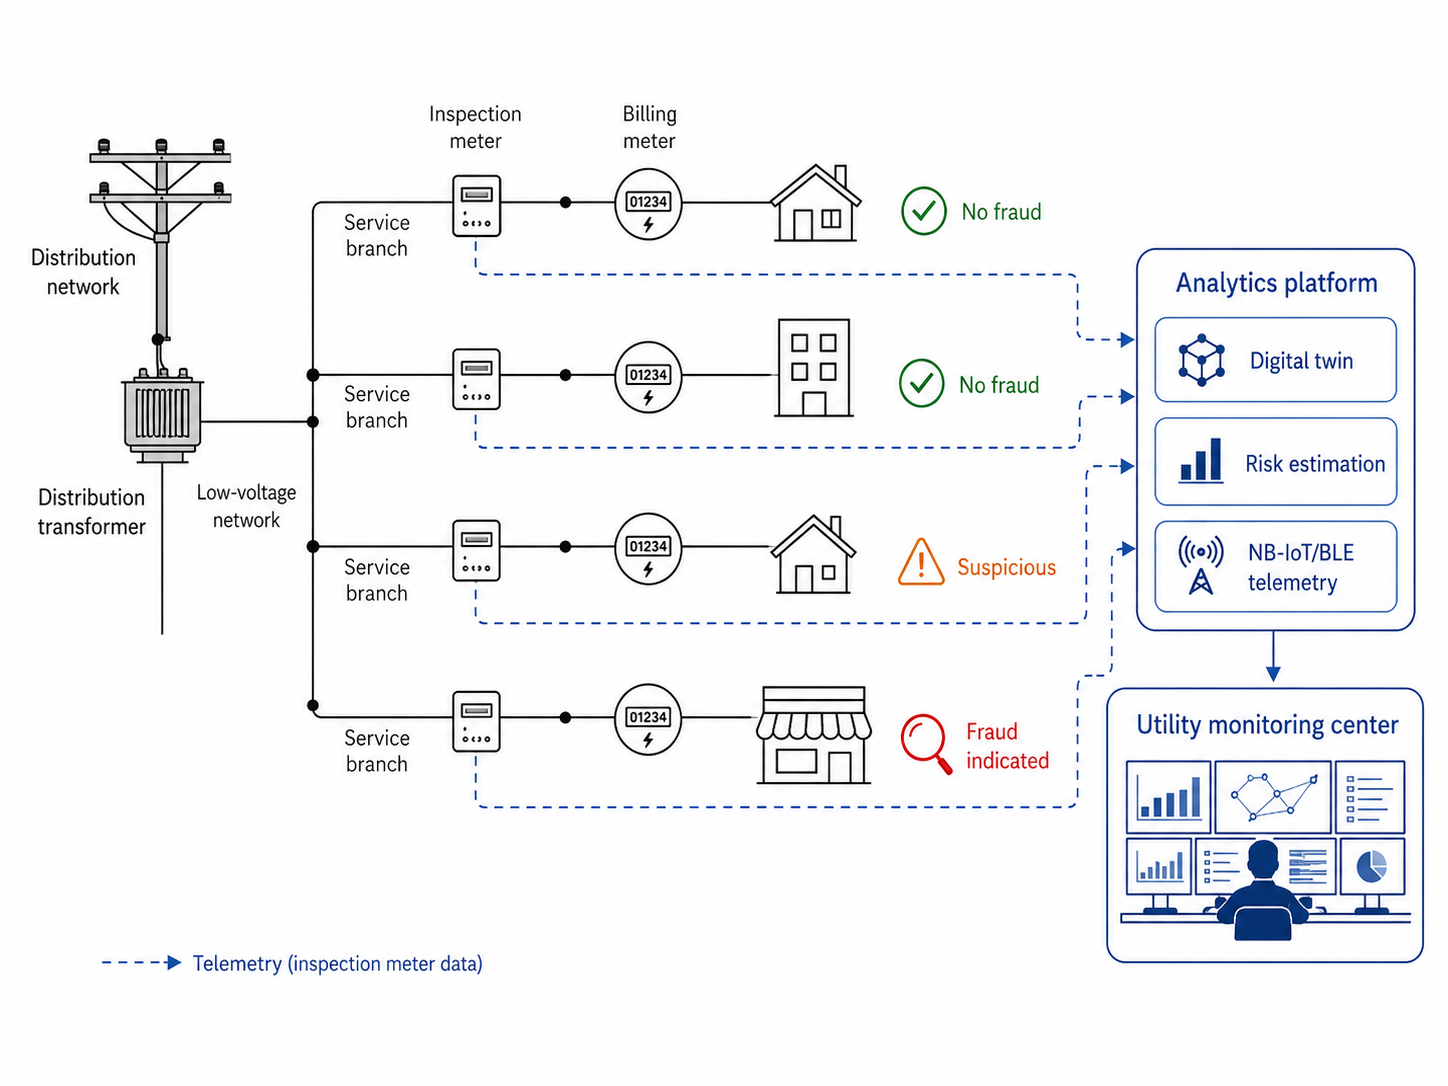
\includegraphics[width=\columnwidth]{fig/topologia_artigo.png}
    \caption{Simplified use-case topology of the proposed forensic telemetry framework.}
    \label{fig:use_case_topology}
\end{figure}

The main contributions are sixfold:
\begin{itemize}
    \item formulating energy-theft monitoring as closed-loop observation control, with telemetry density as a controllable resource and explicit detection and communication-cost objectives;
    \item implementing an application-oriented digital twin that fuses billing and inspection data into contextual theft-risk estimates and explicitly states its current digital-twin scope;
    \item generating heterogeneous, metrologically coherent synthetic fraud scenarios with independent measurement/communication noise and observation modes that are distinct at the native resolution;
    \item proposing adaptive observation windows and empirically characterizing their detection--communication trade-off through a Pareto analysis over fusion and hysteresis parameters;
    \item modeling NB-IoT/BLE communication cost with signaling overhead, retransmission, and latency grounded in reported quality-of-service measurements; and
    \item providing a reproducible seven-scenario comparison of fixed and adaptive policies, complemented by feature importance, an alternative-model comparison, and a scalability benchmark.
\end{itemize}

The remainder of this paper is organized as follows. Section~\ref{sec:related_work} situates the work within the literature and makes explicit the research gap it addresses. Section~\ref{sec:system_model} presents the system model and the formal problem statement. Section~\ref{sec:Materials_Methods} describes the proposed framework, including the reproducible prototype architecture, the digital-twin scope, the synthetic-data methodology, the risk and fusion engines, the communication-cost model, and the complexity analysis. Section~\ref{sec:experimental_campaign} describes the experimental campaign and the comparative evaluation procedure. Section~\ref{sec:Results_Discussion} presents and discusses the results, including a critical assessment of limitations. Section~\ref{sec:Conclusion} concludes the paper.

\section{Related Work}
\label{sec:related_work}
This section positions the proposed framework with respect to three complementary research lines: (i) energy-theft and NTL detection from smart-metering data, (ii) digital twins for smart metering and cyber-physical monitoring, and (iii) adaptive telemetry under communication constraints. The purpose is not to provide an exhaustive systematic review, but to identify which capabilities have already been demonstrated in each line and to clarify the still-unresolved intersection addressed by this work.

\subsection{Bibliographic Search Strategy and Study Selection}
Related literature was identified through structured searches covering 2019--2025, updated through March 2026, organized around three query families: (i) energy theft/NTL, smart meters/AMI, and detection or machine learning; (ii) digital twins, smart grids/meters, and monitoring or telemetry; and (iii) NB-IoT/LPWAN/BLE telemetry with adaptive sampling, reporting, or closed-loop reconfiguration. We made minor syntax adaptations across the consulted bibliographic sources. We retained studies that directly addressed at least one of these three axes and excluded those whose connection to smart metering, energy monitoring, or adaptive observation was only generic. Because this section is intended for technical positioning rather than as a systematic-review contribution, the discussion emphasizes the studies most directly related to the proposed framework; additional measurement and methodological references are introduced where needed.

\subsection{Energy-Theft and Non-Technical-Loss Detection from Smart Metering Data}
Researchers have extensively investigated energy-theft and NTL detection from smart-meter and AMI data using supervised machine learning, deep learning, and ensemble-based methods. These approaches demonstrate that suspicious consumption behavior can be identified with strong classification performance when sufficiently informative historical load series are available \cite{b1,b2,b3,b4,b5,b6}.

Recent work spans CNN and CNN-LSTM architectures \cite{b2,b7}, stacked and boosting-based ensembles \cite{b4,b5,b8}, Transformer-based models designed to capture temporal structure and address class imbalance \cite{b9}, and broader AI-based formulations for theft detection in distribution networks \cite{b10,b11}. Methods aimed at previously unseen fraud patterns have also emerged: Massarani \textit{et al.} \cite{b6} investigate prototype- and ensemble-based zero-day detection, while Blazakis \textit{et al.} \cite{b12} explore quantum machine learning for power-theft detection. Deep reinforcement learning has additionally been investigated for scenarios involving new customers, evolving consumption patterns, zero-day attacks, and newly launched attack strategies \cite{b38}. These directions reinforce, from a detection-model perspective, the behavioral heterogeneity that motivates the fraud-profile modeling adopted in Section~\ref{subsec:synthetic_realism}. Other studies combine clustering, feeder-level aggregation, or contextual customer information to reduce false positives and increase robustness to heterogeneous consumption profiles \cite{b13,b14}.

Despite these advances, most NTL-detection methods operate on pre-collected smart-meter time series with a predefined measurement cadence. Their primary optimization target is therefore the detection model itself rather than the observation process that produces the input data \cite{b2,b5,b6}. This leaves open the question of whether the sensing cadence should itself be dynamically adapted according to the current forensic value of the observed context.

\subsection{Digital Twins for Smart Metering and Cyber-Physical Monitoring}
Digital twins have become an important paradigm for cyber-physical monitoring, prediction, simulation, and operational decision support. In general terms, a digital twin maintains a synchronized virtual representation of a physical asset or process and evolves that representation using data exchanged with the physical counterpart \cite{b15,b16,b17}.

In energy-related applications, digital twins have been used for smart-meter virtualization, real-time monitoring, predictive analysis, secure IoT integration, and energy-system decision support \cite{b18,b19,b20,b21,b22}. Stronger smart-meter-specific examples include Liu \textit{et al.} \cite{b39}, which uses a container-driven architecture to create a virtual dedicated agent (digital twin) for each user-side smart meter and supports cloud/edge service deployment. Bayer and Pruckner \cite{b40} construct a local-energy-system digital twin from real smart-meter data for simulation and decision support. These studies demonstrate that digital twins can provide substantially more than static visualization and can support synchronized services around metering infrastructure.

Outside the specific energy-theft setting, the broader digital-twin literature also includes predictive-maintenance, network-management, and closed-loop adaptive-control applications \cite{b23,b24,b25}. In particular, Liu \textit{et al.} \cite{b25} use a digital twin to support adaptive data-acquisition scheduling in a closed-loop agricultural platform, showing that active sensing is already an established digital-twin capability in other application domains. Within the smart-metering corpus reviewed here, however, the twin is primarily used for virtualization, monitoring, communication services, security analysis, or decision support \cite{b18,b20,b22,b39,b40}. We did not identify a smart-metering framework in which the twin directly controls telemetry density as a function of application-specific energy-theft risk.

\subsection{Adaptive Telemetry and the Still-Unresolved Intersection}
Researchers have investigated adaptive monitoring from several complementary perspectives. Qaddoori and Ali \cite{b26} support iterative updating of smart-meter anomaly models, while Raeiszadeh \textit{et al.} \cite{b27} adapt industrial-IoT anomaly detection to concept drift in streaming data. From a communication perspective, El Sayed \textit{et al.} \cite{b28} combine adaptive compression and anomaly detection for distributed digital-twin use cases, reducing transport-network requirements while preserving monitoring capability.

In smart-metering and LPWAN scenarios, researchers have also proposed adaptive transmission policies that adjust reporting intervals based on observed data dynamics. Al-Sammak \textit{et al.} \cite{b29}, for example, adapt transmission timing for LoRaWAN and NB-IoT smart-meter telemetry and report substantial reductions in packet transmissions and communication-related energy consumption. Related NB-IoT work demonstrates the feasibility of remote metering and power-system status monitoring over lightweight wide-area telemetry links \cite{b30,b31}. Measurement- and model-based studies further provide experimentally grounded ranges and trends for latency, coverage, repetitions, connection-management behavior, and energy--latency trade-offs in NB-IoT deployments \cite{b32,b33,b34,b35}. These results motivate the network-representative, rather than carrier-specific, communication-cost assumptions adopted in Section~\ref{subsec:network_cost}.

Taken together, the reviewed literature reveals a separation among the three research directions. Energy-theft studies improve detection models while operating on predefined telemetry streams; adaptive-telemetry studies primarily optimize communication, energy efficiency, model adaptation, or generic monitoring quality without considering theft-oriented forensic utility; and smart-meter digital twins focus mainly on virtualization, monitoring, communication services, and decision support. Within the reviewed corpus, we did not identify a framework that jointly uses contextual theft-risk estimation, explicit digital-twin state and decision logic, and adaptive telemetry density within the same closed observation-control loop. This is the intersection addressed by the present work: sensing density is treated as a controllable resource, and the digital twin uses contextual risk as the control signal for risk-driven forensic observability over NB-IoT telemetry.

\subsection{Comparative Summary}

\begin{table*}[!ht]
\centering
\caption{Positioning of this work relative to the closest literature}
\label{tab:rw_comparison}
\begin{tabular}{|p{2.4cm}|p{4.8cm}|p{3.3cm}|p{3.3cm}|p{1.7cm}|}
\hline
\textbf{Research line} & \textbf{Core contribution} & \textbf{Typical assumption} & \textbf{Main limitation relative to this work} & \textbf{Representative references} \\
\hline
Energy theft / NTL detection & Theft detection from smart-meter or AMI data using ML, DL, ensembles, anomaly models, QML, or RL & Predefined telemetry stream & Does not treat observation density as a theft-risk-driven control variable & \cite{b1,b2,b4,b5,b6,b7,b8,b9,b12,b13,b14,b38} \\
\hline
Digital twins for smart metering and energy systems & Virtualization, synchronized monitoring, cloud/edge services, simulation, and decision support & Twin supports metering or energy-system services & Smart-meter twins rarely control sensing density according to forensic risk & \cite{b18,b20,b21,b22,b39,b40} \\
\hline
Adaptive telemetry / adaptive monitoring & Dynamic reporting, model adaptation, compression, and NB-IoT communication-efficiency characterization & Adaptation driven mainly by communication, energy, or generic monitoring objectives & Does not optimize telemetry density for theft-oriented forensic utility & \cite{b26,b27,b28,b29,b30,b31,b32,b33,b34,b35} \\
\hline
This work & Contextual theft-risk estimation with digital-twin-guided adaptive observation for NB-IoT forensic telemetry and an explicit communication-cost model & Observation density is controllable & Balances detection capability and communication cost; field validation remains future work & This article \\
\hline
\end{tabular}
\end{table*}

Table~\ref{tab:rw_comparison} summarizes the positioning of the present work with respect to the three closest research lines. The distinguishing contribution is not the isolated use of machine learning, a digital twin, or adaptive telemetry, all of which have precedents in the literature. Rather, it integrates them into a closed observation-control loop in which contextual energy-theft risk determines the future density of forensic telemetry, and the resulting detection--communication trade-off is characterized explicitly.


\section{System Model and Problem Formulation}
\label{sec:system_model}
This work formulates the problem as an adaptive observation-control problem in forensic telemetry. At each potential acquisition instant $t$, the system has access to an observational state $s_t$ summarizing the electrical, temporal, operational, and historical conditions of the monitored asset. In the current prototype, $s_t$ includes, among other variables, relative power divergence, accumulated energy difference, moving averages of divergence over real-time windows, hourly recurrence, alarm score, and the operational-integrity signals \textit{link} and \textit{heartbeat}. Based on $s_t$, the digital twin selects an action $a_t \in \mathcal{A} = \{\text{basal},\, \text{moderate},\, \text{aggressive}\}$, where each action induces a distinct capture interval $\Delta(a_t) \in \{60, 15, 5\}$ minutes, respectively.

The system dynamics are partially controlled: the action taken at time $t$ alters the future observation density, which changes the information available at subsequent times. This distinguishes the problem from static classification over a fixed sample set, since the decision policy affects the observation process that will feed future decisions.

Let $o_t(a_{1:t}) \in \{0,1\}$ denote whether the forensic device emits (is observed) at instant $t$ under the capture schedule induced by the action history up to $t$ (Algorithm~\ref{alg:closed_loop_twin}), and let $p_t^{(d)}(s_t) \in [0,1]$ denote the fused decision probability produced by the twin (Section~\ref{subsec:fusao}). Let $y_t \in \{0,1\}$ denote the (unobserved, ground-truth) theft-activity indicator and $\tau$ the decision threshold. The detection capability of a policy over a horizon of $T$ instants is defined as
\begin{equation}
D\big(s_{1:T}, a_{1:T}\big) =
\frac{1}{\sum_{t=1}^{T} y_t}
\sum_{t=1}^{T}
y_t \cdot o_t(a_{1:t}) \cdot
\mathbb{I}\left[p_t^{(d)}(s_t)\ge\tau\right],
\label{eq:detection_capability}
\end{equation}
where $\mathbb{I}[\cdot]$ denotes the indicator function, equal to 1 when the enclosed condition is true and 0 otherwise. Thus, $D$ represents the fraction of all ground-truth theft instants on the native-resolution horizon that are both observed and correctly flagged. A theft instant with $y_t=1$ that is not sampled ($o_t=0$), as well as an observed theft instant whose decision probability remains below $\tau$, contributes to the denominator but not to the numerator and is therefore a false negative at the policy level. Hence, Eq.~\eqref{eq:detection_capability} is precisely the recall of the induced observation-and-detection policy, made explicit as a function of the state trajectory (through $p_t^{(d)}$) and the action trajectory (through $o_t$). Equation~\eqref{eq:detection_capability} applies to horizons containing at least one ground-truth theft instant ($\sum_{t=1}^{T} y_t>0$). For theft-free horizons, policy-level recall is undefined; the zero values used in the campaign-wide aggregate results are an explicit reporting convention rather than evaluations of Eq.~\eqref{eq:detection_capability}.

Let $b_t(s_t)$ denote the per-event communication cost in bytes returned by the transport-cost model of Section~\ref{subsec:network_cost}, which depends on the operational context captured in $s_t$ (link and heartbeat state) and on whether a fresh NB-IoT connection must be established. The communication cost of a policy is
\begin{equation}
C\big(s_{1:T}, a_{1:T}\big) = \sum_{t=1}^{T} o_t(a_{1:t}) \cdot b_t(s_t).
\label{eq:communication_cost}
\end{equation}
The objective of the digital twin is to select an action sequence that maximizes
\begin{equation}
U\big(a_{1:T}\big) = \lambda_1 \cdot D\big(s_{1:T}, a_{1:T}\big) - \lambda_2 \cdot C\big(s_{1:T}, a_{1:T}\big),
\label{eq:utility}
\end{equation}
where $\lambda_1,\lambda_2\geq 0$ express the relative importance of forensic sensitivity and communication efficiency. Searching directly over the space of action sequences is combinatorial ($|\mathcal{A}|^T$) and would require selecting a specific $(\lambda_1,\lambda_2)$ pair a priori. Equation~\eqref{eq:utility} therefore provides a conceptual formulation of the operational objective, with $D$ explicitly representing policy-level recall as defined in Eq.~\eqref{eq:detection_capability}.

For the empirical trade-off analysis, however, this study does not directly optimize Eq.~\eqref{eq:utility}. Instead, Section~\ref{subsec:tradeoff_resolution} restricts the search to the low-dimensional, interpretable policy-parameter family $\Theta=(\alpha,\tau_{\mathrm{moderate}},\tau_{\mathrm{high}})$, comprising the fusion weight and the two hysteresis thresholds that determine the induced action sequence for a given observation trace. Within this parameter family, we adopt the F1-score as the empirical detection-performance score because it jointly reflects precision and recall, while $C(\Theta)$ represents communication cost. The evaluated configurations therefore generate empirical points in the $\bigl(F_1(\Theta),C(\Theta)\bigr)$ plane.

The non-dominated subset of these points constitutes the empirical Pareto frontier reported in Section~\ref{subsec:tradeoff_resolution}. This frontier summarizes the detection--communication trade-offs available within the evaluated parameter grid: moving to another non-dominated operating point can improve one objective only at the expense of the other. It does not imply that every frontier point is the solution of Eq.~\eqref{eq:utility} for some $(\lambda_1,\lambda_2)$ pair, nor does it constitute a proof of global optimality over the full action-sequence space. Rather, it provides a decision-support representation from which an operating configuration can be selected according to deployment-specific preferences.

Since Eq.~\eqref{eq:utility} is not directly observable during deployment, the experimental evaluation approximates $D$ and $C$ using precision, recall, F1-score, and a critical-slot metric for the detection side, and communication bytes, latency, and retransmission counts for the cost side (Section~\ref{subsec:metrics}). Under this formulation, the framework does not merely classify theft versus non-theft; it decides when it is worthwhile to increase the temporal resolution of observation, with the risk probability estimated by the twin's engines acting as the control signal that governs telemetry density.

\section{Materials and Methods}
\label{sec:Materials_Methods}
\subsection{Methodological Overview}
This section describes the experimental framework implemented to evaluate energy-theft probability classification with adaptive observation control in an NB-IoT-based forensic telemetry scenario. The methodological objective is not merely to estimate risk from previously available telemetry, but to build an application-oriented digital twin that interprets context, determines observation density, and locally updates the capture regime throughout the experiment.

The framework was built as a reproducible local-execution prototype, fully implemented in Python, with simplified installation, SQLite persistence, and command-line execution. This design choice had two main motivations. First, it ensured that the experiments reported in the paper could be reproduced without mandatory dependence on external infrastructure. Second, it made the digital-twin architecture explicit in code before integrating with real data, an NB-IoT broker, and real-time BLE contingency.

Conceptually, the framework is organized into seven layers: data ingestion, contextual enrichment, risk engines, explicit digital-twin state, policy orchestration, a local closed-loop runtime with simulated devices, and a communication-cost/complexity evaluation layer. Unlike a static classification pipeline, the current implementation contains explicit entities for twin state, decision, command plan, transport cost, and execution of the perception-decision-action cycle.

\subsection{System Under Consideration and Firmware-Integration Assumptions}
\label{subsec:System_Under_Consideratio}
The target system consists of a billing meter and a discrete forensic telemetry device installed in parallel with the monitored installation. The forensic device is an already-implemented, certified embedded product, compliant with the electromagnetic-compatibility immunity requirements of IEC 61000-4-4 (electrical fast transient/burst), IEC 61000-4-5 (surge), IEC 61000-4-6 (conducted radio-frequency disturbances), and IEC 61000-4-11 (voltage dips, short interruptions, and variations), and engineered with a metrological error class equivalent to that of the billing meter it monitors, so that forensic-versus-billing divergence reflects a genuine metering discrepancy rather than an artifact of instrument-class mismatch. The device is intentionally discreet, so that its presence is not readily apparent to the customer whose installation is being inspected. It is assumed that the embedded layer already provides instantaneous electrical quantities, historical profiles, alarms, local persistence, and telemetry parameters remotely configurable via NB-IoT, with BLE available as a local contingency channel. The device is powered by the monitored installation's network connection and is therefore available full-time; device energy consumption is outside the scope of this study; the operational cost that matters to the distribution utility, and that this paper targets, is the volume and cost of transmitted data.

At this stage, integration with the physical layer is represented by synthetic traces semantically aligned with the firmware domain. The field names used in data generation and processing preserve this semantic proximity without breaking the logical architecture of the framework: the electrical quantities follow the instantaneous-metrology naming used by the firmware (e.g., \texttt{voltage\_rms}, \texttt{active\_power}, \texttt{power\_factor}), and the alarm flags follow the firmware's alarm-manager naming (e.g., \texttt{alarm\_overvoltage}, \texttt{alarm\_overcurrent}).

\subsection{Digital-Twin Criteria and Scope}
\label{subsec:twin_criteria}
Because the term ``digital twin'' is used inconsistently across the literature, this subsection makes explicit which criteria the implementation satisfies, and to what degree, rather than asserting the label without justification. Following the broader cyber-physical-systems view of digital twins as closed-loop mechanisms for monitoring, prediction, and control \cite{b15,b16,b24}, four criteria are considered:

\begin{enumerate}
    \item \textit{State persistence.} The \textit{ForensicTwin} entity maintains an explicit, event-indexed state (current observation mode, capture period, mode-dwell count, last decision probabilities, and last command) that is snapshotted and persisted at every observed event, independent of any single classification call. The current implementation fully satisfies this criterion.
    \item \textit{Bidirectional synchronization with a physical asset.} The twin both receives evidence from, and issues reconfiguration commands to, the forensic device's emission schedule. In the present study, this synchronization loop is materialized with a locally simulated device (\textit{MockForensicDevice}) and transport (\textit{MockTransport}), because the physical forensic device described in Section~\ref{subsec:System_Under_Consideratio} already exists and is certified. Still, end-to-end NB-IoT/BLE integration with the twin software is planned future work. This criterion is therefore satisfied at the software-architecture level and in a local closed loop, but it has not yet been validated against a physically deployed radio link.
    \item \textit{Closed-loop decision-making.} The action selected at time $t$ (Section~\ref{sec:system_model}) changes the future observation density, which changes the evidence available to subsequent decisions. Algorithm~\ref{alg:closed_loop_twin} and the runtime evidence reported in Section~\ref{sec:Results_Discussion} (distinct sample counts per observation mode, issued reconfiguration commands, transport-delivery records) demonstrate that this loop is exercised, not merely described. This criterion is fully satisfied within the local runtime.
    \item \textit{Active sensing/control layer, not a passive monitor.} In contrast to the smart-metering digital-twin studies reviewed in Section~\ref{sec:related_work}, which primarily emphasize virtualization, monitoring, communication services, security analysis, and decision support \cite{b18,b20,b22,b39,b40}, the twin in this work is the entity that decides the telemetry density itself according to the current forensic-risk context. This is the paper's central architectural claim and is fully satisfied within the implemented local runtime.
\end{enumerate}

In summary, this study implements the software layer of an application-oriented digital twin. Three of the four criteria are fully realized within the local closed-loop runtime. In contrast, bidirectional synchronization with the physical forensic device is currently closed only through a reproducible simulation rather than through a deployed NB-IoT/BLE radio link. This scoping is stated explicitly rather than left implicit, and is treated further as a threat to validity in Section~\ref{subsec:limitations}.

\subsection{Implemented Digital-Twin Architecture}
\label{subsec:Implemented_DT_Architecture}
The framework's core is the \textit{ForensicTwin} digital twin, implemented as a software entity with its own state and event-oriented updates. At each observed event, the twin receives a \textit{TwinObservation}, produced by temporally fusing forensic measurements, billing measurements, and alarm events. This observation contains the electrical, temporal, operational, and alarm-related attributes required for risk inference.

A \textit{DecisionEngine} operates on this observational state and transforms the current context into a probabilistic risk decision. The engine uses two evidence sources: a rule-based contextual baseline and a supervised logistic-regression baseline. Rather than assuming a single fixed combination rule, the framework supports three explicit probability-fusion strategies: \textit{weighted}, \textit{conservative\_max}, and \textit{context\_aware} (Section~\ref{subsec:fusao}).

The output of the \textit{DecisionEngine} is consumed by a \textit{PolicyOrchestrator}, which converts the decision into an observational action. This action is formalized in the \textit{TelemetryReconfigurationDecision} structure, which represents the command plan issued by the digital twin. Among other fields, the command specifies the monitored asset identifier, selected mode, capture interval, decision probability, probability source, textual justification, and preferred transport.

To materialize the closed loop in a local environment, the framework further uses three simulation components: \textit{MockForensicDevice}, \textit{MockBillingMeter}, and \textit{MockTransport}. The first simulates the forensic device and adjusts its future emission cadence based on the received command. The second provides the billing reference. The third simulates local command delivery, preferentially using NB-IoT and falling back to BLE in degraded scenarios (which, in a real system, would require a local operator with a BLE-enabled device), using the communication-cost model of Section~\ref{subsec:network_cost}. \textit{SimulationRunner} handles the integrated execution of these components and explicitly implements the framework's local closed loop.

\begin{figure*}[!t]
      \centering
      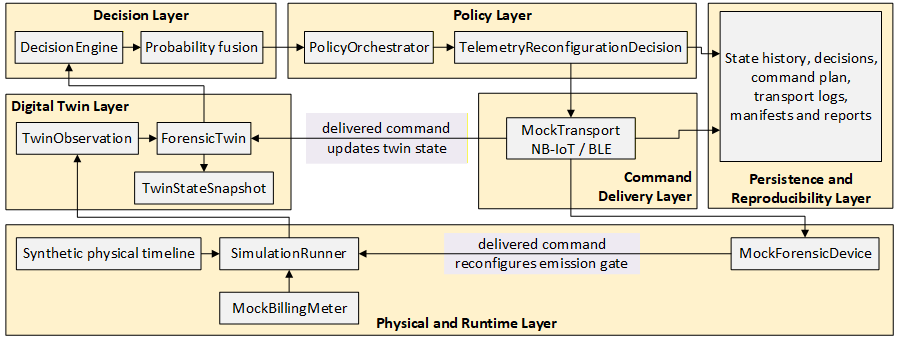
\includegraphics[width=0.9\textwidth]{fig/framework_architecture2.png}
      \caption{Closed-loop architecture of the proposed digital-twin framework.}
      \label{fig:framework_architecture}
\end{figure*}

Fig.~\ref{fig:framework_architecture} summarizes the implemented framework architecture. As shown, the core of the system is composed of the \textit{ForensicTwin}, the decision layer \textit{DecisionEngine}, the policy-orchestration layer \textit{PolicyOrchestrator}, and the explicit command-plan formalization \textit{TelemetryReconfigurationDecision}. These components operate jointly with the local runtime and the simulated devices, materializing a closed loop in which the twin's decision changes the future observation density.

\subsection{Formalization of the Local Closed Loop}
\label{subsec:Local_Closed_Loop}
The local runtime executes the following cycle in temporal order:
\begin{enumerate}
    \item traverses the synthetic physical timeline at native resolution;
    \item checks, through the \textit{MockForensicDevice}, whether the current event should be emitted according to the active capture interval;
    \item whenever the event is emitted, constructs a \textit{TwinObservation};
    \item evaluates the observation with the \textit{DecisionEngine};
    \item applies a probabilistic fusion strategy;
    \item generates a \textit{TelemetryReconfigurationDecision} with the \textit{PolicyOrchestrator};
    \item delivers the command through the \textit{MockTransport}, which resolves NB-IoT/BLE selection and the resulting cost/latency;
    \item applies the command to the \textit{ForensicTwin} and to the \textit{MockForensicDevice}; and
    \item updates the twin state and the future emission cadence.
\end{enumerate}

\begin{algorithm}[!ht]
\caption{Local closed loop of the digital twin}
\label{alg:closed_loop_twin}
\begin{algorithmic}[1]
\REQUIRE Synthetic timeline $\mathcal{X}$, twin $T$, forensic device $D$, billing meter $B$, transport $L$
\FORALL{instant $x_t \in \mathcal{X}$}
    \IF{$D.\text{should\_emit}(x_t)$}
        \STATE $o_t \gets \text{build\_observation}(x_t, B)$
        \STATE $d_t \gets T.\text{update}(o_t)$
        \STATE $c_t \gets \text{PolicyOrchestrator}(d_t)$
        \STATE $L.\text{deliver}(c_t)$
        \STATE $T.\text{apply}(c_t)$
        \STATE $D.\text{apply}(c_t)$
    \ENDIF
\ENDFOR
\end{algorithmic}
\end{algorithm}

This modeling choice is important because it shifts the experiment from a simple offline evaluation on fixed samples to an environment in which observability itself becomes a consequence of the twin's decisions. Although the physical loop is local and simulated, the logical structure of perception, inference, action, and feedback is already explicitly materialized, and its runtime cost is characterized in Section~\ref{subsec:complexity}.

\subsection{Native Temporal Resolution and Observation Modes}
\label{subsec:native_resolution}
The native acquisition grid of the synthetic physical timeline is set to 5 minutes, an exact common divisor of the three observation-mode capture periods used by the policy orchestrator: \textit{basal} (60 minutes), \textit{moderate} (15 minutes), and \textit{aggressive} (5 minutes). This choice is methodologically necessary: the forensic-device emission gate (Algorithm~\ref{alg:closed_loop_twin}, line 2) can never emit faster than data exists on the underlying timeline, so a native resolution coarser than the finest observation mode would make that mode indistinguishable, at the data level, from any mode with an equal or coarser capture period. With the 5-minute native grid, \textit{aggressive} observes every native tick, \textit{moderate} observes every third tick, and \textit{basal} observes every twelfth tick, so the three modes induce genuinely different observation densities; this property is verified directly by a unit test that drives the device emission gate over a synthetic 5-minute-spaced timeline and asserts the expected 12:4:1 emission ratio across aggressive, moderate, and basal modes.

A direct consequence of this resolution choice is that a fixed policy reporting on a 15-minute cadence (\textit{fixed\_short}, retained from earlier campaigns as an intermediate, realistic fixed-cadence baseline) is a genuinely sparser policy than the native acquisition grid, and can therefore no longer serve as a proxy for "dense monitoring." Accordingly, this study introduces a fourth policy, \textit{fixed\_dense}, which reports at the native 5-minute resolution and is used throughout Section~\ref{sec:Results_Discussion} as the empirical ceiling against which the detection performance of every other policy, fixed or adaptive, is compared.

\subsection{Synthetic Data Generation: Metrological Coherence, Realistic Noise, and Heterogeneous Fraud Profiles}
\label{subsec:synthetic_realism}
The experimental campaign is built upon seven controlled synthetic scenarios: normal operation, persistent theft, peak-hour theft, nighttime theft, intermittent nighttime theft, disturbance without theft, and a degraded-link scenario without theft. Each scenario covers seven days of observation at the native 5-minute resolution. Generation is deterministic, with explicit random seeds, producing three temporal streams per scenario: forensic-device measurements, billing-meter measurements, and alarm events.

The synthetic traces preserve metrological coherence among voltage, current, active power, reactive power, apparent power, power factor, and accumulated energies: at each interval, RMS voltage and active power are first defined from the scenario load profile, after which the power factor is sampled within a plausible range and used to consistently derive apparent power, reactive power, and RMS current; active and reactive energies are then accumulated over time according to the native time step. This ensures that the risk features extracted by the framework correspond to electrically plausible observational discrepancies rather than to arbitrary differences between artificial time series.

Two properties of the data-generation process are essential to the internal validity of the classification problem addressed in this paper, and we make them explicit here because they directly determine whether the reported detection metrics are meaningful or an artifact of how the labels were produced. First, we do not treat the discrepancy between the forensic and billing readings as a single deterministic function of a scenario-level theft ratio. Independent, theft-unrelated noise sources are added to both meters: per-meter metrological noise (approximately 1.2\% relative standard deviation, applied independently to the forensic and billing active-power readings before the internally consistent electrical quantities are derived), transient communication/reporting glitches (occurring with 3\% per-tick probability, at a magnitude comparable to a low-severity theft event, and applied at random to either meter), and legitimate but erratic load surges (occurring with 1.5\% per-tick probability, representing events such as a large appliance motor start) that are independent of theft activity. The out-of-bounds-power alarm, which in an earlier version of this framework was derived directly from the forensic-versus-billing gap, is redefined here using only the forensic meter's own reading against a fixed contracted-demand ceiling, so that no alarm used as a classification feature can, by construction, encode the detection label.

Second, theft severity and temporal behavior are made heterogeneous rather than uniform, reflecting the diversity of fraud strategies reported in practice, from constant partial diversion to brief, near-total diversion confined to specific hours. Each active theft tick is assigned one of four fraud profiles: \textit{stealth} (a small, 5\%-to-11\% diversion ratio, deliberately close to the sensor-noise floor), \textit{partial\_constant} (a stable 15\%-to-25\% diversion), \textit{partial\_variable} (an 8\%-to-40\% diversion that depends on the hour of day, more pronounced during peak hours), and \textit{full\_diversion} (a 55\%-to-88\% diversion confined to short windows, occasionally accompanied by a probabilistic, non-deterministic current-imbalance artifact representative of a bypass connection). In addition, for the two scenarios whose theft window would otherwise recur at an identical hour of day on every single day of the observation period (\textit{peak\_theft} and \textit{night\_theft}), theft occurrence is made probabilistic per day (82\% of days), rather than certain, so that a classifier cannot achieve perfect separation from the hour-of-day feature alone, independent of any electrical evidence.

\subsection{Feature Construction and Risk Engines}
Risk features are constructed from four evidence groups, all derived from the synthetic streams described above. The first group corresponds to the electrical divergence between the forensic and billing measurements, including relative active-power divergence and moving averages/maxima of that divergence computed over real-time windows (60 and 120 minutes, respectively) rather than fixed sample counts, so that their meaning is independent of the native acquisition resolution. The second group corresponds to temporal context (hour of day, day of week, and the historical recurrence of suspicious divergence within the same hour-of-day slot). The third group corresponds to alarm context (out-of-bounds power, overcurrent, undervoltage, and overvoltage), aggregated into a single alarm score. The fourth group comprises the operational-integrity signals \textit{link} and \textit{heartbeat}, which distinguish low observability caused by communication degradation from a genuinely suspicious electrical context.

Two risk engines operate on this feature set. The first is a rule-based baseline designed for auditability and interpretability, explicitly combining divergence magnitude, temporal persistence, alarm context, and operational integrity into a comprehensible and traceable risk score. The second is a supervised baseline based on logistic regression, with numerical preprocessing and an explicit constant-prediction fallback for scenarios whose training split contains a single class (as occurs, by construction, in the \textit{normal}, \textit{persistent\_theft}, \textit{disturbance\_without\_theft}, and \textit{degraded\_link\_no\_theft} scenarios, where the classification task is degenerate rather than an artifact of leakage). The rule-based output is normalized to the interval $[0,1]$ and used as a fusion-compatible risk score; it is not interpreted as a calibrated posterior probability.

To probe whether additional nonlinear model capacity provides a benefit, and to quantify which features drive the logistic-regression baseline's decisions, this study additionally trains a two-hidden-layer multilayer perceptron (16 and 8 units, respectively) on the same feature set and the same train/test split, and reports standardized logistic-regression coefficients together with permutation feature importance (20 repetitions, F1-scoring) on the held-out test split. Neither the alternative model nor the importance analysis feeds the twin's decision loop; both are reporting-only diagnostics computed alongside the pipeline that produces the twin's \textit{supervised\_probability}.

\subsection{Probability-Fusion Strategies}
\label{subsec:fusao}
\begin{table}[ht]
\centering
\caption{Legend of the mathematical symbols used in the probability-fusion formulation.}
\label{tab:fusion_symbols}
\begin{tabular}{p{1.3cm} p{6.38cm}}
\hline
\textbf{Symbol} & \textbf{Meaning} \\
\hline
$t$ & Temporal index of the observed event \\
$p_t^{(r)}$ & Normalized risk score produced by the rule-based engine at time $t$ \\
$p_t^{(s)}$ & Risk probability estimated by the supervised engine at time $t$ \\
$p_t^{(d)}$ & Final probability used by the digital-twin decision layer at time $t$ \\
$\alpha$ & Weight assigned to the rule-based component in the \textit{weighted} strategy \\
$1-\alpha$ & Weight assigned to the supervised component in the \textit{weighted} strategy \\
$\mathcal{C}_t$ & Observational context at time $t$, composed of electrical, temporal, operational, and alarm evidence \\
$w_r(\mathcal{C}_t)$ & Contextual weight assigned to the rule-based engine in the \textit{context\_aware} strategy \\
$w_s(\mathcal{C}_t)$ & Contextual weight assigned to the supervised engine in the \textit{context\_aware} strategy \\
$\max(\cdot)$ & Maximum operator, used to select the highest probability among two sources \\
\hline
\end{tabular}
\end{table}

Let $p_t^{(r)} \in [0,1]$ denote the normalized risk score produced by the rule-based engine at time $t$, and let $p_t^{(s)} \in [0,1]$ denote the probability estimated by the supervised baseline. The fusion layer produces a single decision probability $p_t^{(d)} \in [0,1]$, which the digital twin uses as the control signal to select the subsequent observation regime. Three fusion strategies are considered.

In the \textit{weighted} strategy,
\begin{equation}
p_t^{(d)} = \alpha\, p_t^{(r)} + (1-\alpha)\, p_t^{(s)}, \qquad \alpha \in [0,1].
\label{eq:weighted_fusion}
\end{equation}
In the current prototype, $\alpha = 0.6$ is used to favor the interpretability and robustness of the rule-based component without discarding the additional information provided by the supervised baseline; Section~\ref{subsec:tradeoff_resolution} reports where this choice falls relative to the empirical Pareto frontier over $\alpha$ and the decision thresholds.

In the \textit{conservative\_max} strategy,
\begin{equation}
p_t^{(d)} = \max\left(p_t^{(r)},\, p_t^{(s)}\right).
\label{eq:conservative_fusion}
\end{equation}
This corresponds to a conservative stance for inspection purposes, in which the final decision inherits the highest-risk indication between the two sources, tending to increase system sensitivity at the potential cost of denser observations and higher communication volume.

In the \textit{context\_aware} strategy, the fusion weights depend on the electrical and operational context observed at time $t$. Let $c_t \in \{\text{electrical-dominant},\, \text{temporal-dominant},\, \text{balanced}\}$ be assigned as electrical-dominant if active alarms are present or electrical divergence is strong, temporal-dominant if relevant temporal recurrence is present without dominant electrical evidence, and balanced otherwise. The final probability is
\begin{equation}
p_t^{(d)} = w_r(c_t)\, p_t^{(r)} + w_s(c_t)\, p_t^{(s)}, \qquad w_r(c_t) + w_s(c_t) = 1,
\label{eq:context_fusion}
\end{equation}
with greater weight assigned to the rule-based engine when $c_t = \text{electrical-dominant}$, greater weight assigned to the supervised component when $c_t = \text{temporal-dominant}$, and an intermediate combination otherwise.

\begin{table*}[ht]
\centering
\caption{Comparison of the probability-fusion strategies considered in the framework.}
\label{tab:fusion_strategies}
\begin{tabular}{p{2.0cm} p{4.2cm} p{4.4cm} p{4.6cm}}
\hline
\textbf{Strategy} & \textbf{Mathematical definition} & \textbf{Operational interpretation} & \textbf{Main methodological risk} \\
\hline
\textit{weighted} & Eq.~\eqref{eq:weighted_fusion}, with $\alpha \in [0,1]$ and greater weight assigned to the rule-based component & Robust compromise in terms of average sensitivity, balancing interpretability and generalization without exclusively privileging a single source & May excessively smooth critical evidence if the weight is poorly calibrated, reducing sensitivity to short or highly localized events \\
\textit{conservative\_max} & Eq.~\eqref{eq:conservative_fusion} & Conservative inspection-oriented policy, prioritizing the highest suspicion available among the two sources & Tends to increase sensitivity at the cost of higher false-alert rates and higher communication cost due to more frequent densification \\
\textit{context\_aware} & Eq.~\eqref{eq:context_fusion}, with weights defined by the observational context & Semantic adaptation to the type of evidence, prioritizing alarms and strong electrical signals or temporal recurrence and historical patterns & Depends on the quality of contextual modeling; poorly specified switching rules may introduce instability or bias \\
\hline
\end{tabular}
\end{table*}

Tables~\ref{tab:fusion_symbols} and~\ref{tab:fusion_strategies} summarize the symbols used in the fusion layer and the methodological differences among the three strategies, respectively. Under this formulation, the observation policy is governed by a decision variable explicitly built from multiple evidence sources, making fusion part of the experimental method rather than an implementation detail. Section~\ref{subsec:results_fusion_ablation} reports a controlled ablation of the fusion strategies.

\subsection{NB-IoT/BLE Communication-Cost Model}
\label{subsec:network_cost}
We model the communication cost of each transmission explicitly rather than approximating it with a flat bytes-per-sample proxy. A transmission over NB-IoT incurs a fixed payload ($64$ bytes), a signaling-overhead term for connection establishment, and a probabilistic number of retransmissions. If the elapsed time since the last NB-IoT transmission exceeds a 15-minute connection-reuse window, we assume a fresh radio-resource-control-style connection and add $40$ bytes of signaling overhead; otherwise, we reuse the ongoing connection at no additional signaling cost. Retransmissions follow a truncated process (at most three attempts) with a per-attempt continuation probability of $0.04$ under nominal link/heartbeat conditions and $0.35$ under degraded conditions; each retransmission adds one payload's worth of bytes and a latency penalty of $900$ ms on top of a $1600$ ms base latency. When the link or heartbeat signal indicates degraded connectivity, the model falls back to BLE, with a fixed overhead of $20$ bytes and a base latency of $120$ ms, consistent with the local-contingency role described in Section~\ref{subsec:Implemented_DT_Architecture}.

The numeric parameters are engineering approximations grounded in reported NB-IoT measurement studies rather than a carrier-specific claim. The $1600$ ms base latency lies within the sub-2-second outdoor and sub-8-second deep-indoor round-trip latencies measured for an NB-IoT-based smart-grid control application on a commercial network \cite{b32}. The connection-setup overhead reflects a legacy (non-optimized) control-plane connection, consistent with the small-message regime targeted by Release-15 Early Data Transmission, which is reported to reduce transmission delay by more than 50\% for uplink messages under approximately 97 bytes on a comparable smart-metering NB-IoT deployment \cite{b33}; because this system's payload (64 bytes) falls within that small-message regime, the reported overhead should be read as a conservative, non-optimized baseline. The asymmetry between nominal and degraded retransmission probabilities reflects the coverage-dependent repetition behavior characterized by systematic quality-of-service measurements of commercial NB-IoT deployments \cite{b34}. Critically, this model is applied consistently across every policy considered in this study, including the fixed policies, so that the reported communication-bytes figures for \textit{fixed\_long}, \textit{fixed\_short}, \textit{fixed\_dense}, and \textit{adaptive} are comparable on a like-for-like basis rather than derived from different cost assumptions. Consistent with Section~\ref{sec:introduction}, no energy-consumption term is included in this model, since the forensic device is mains-powered.

\subsection{Detection-vs-Communication-Cost Trade-off Resolution}
\label{subsec:tradeoff_resolution}
Rather than leaving the fusion weight $\alpha$ and the hysteresis thresholds $\tau_{\text{moderate}}, \tau_{\text{high}}$ as fixed, unjustified constants, this study resolves their trade-off empirically. A grid search is performed over $\alpha \in \{0.2, 0.4, 0.5, 0.6, 0.8\}$, $\tau_{\text{moderate}} \in \{0.20, 0.25, 0.30, 0.35\}$, and $\tau_{\text{high}} = \tau_{\text{moderate}} + \Delta$ with margin $\Delta \in \{0.20, 0.30, 0.40\}$ (capped at $0.95$), yielding 60 parameter combinations, each evaluated on three representative theft scenarios (\textit{intermittent\_evening}, \textit{peak\_theft}, and \textit{night\_theft}, chosen for computational tractability of the grid search since they are the scenarios in which the observation policy has a non-degenerate detection task) through the full closed-loop runtime of Section~\ref{subsec:Local_Closed_Loop}. The non-dominated subset of the resulting $\bigl(F_1(\Theta), C(\Theta)\bigr)$ points, aggregated by mean across the three scenarios, constitutes the empirical Pareto frontier. This procedure follows the same multiobjective, Pareto-front methodology used to characterize the energy-latency trade-off of NB-IoT power-saving features \cite{b35}, but applies it here to the detection-cost trade-off. This is presented as an empirical, reproducible resolution of the trade-off, not a formal proof of global optimality across the full action-sequence space of Section~\ref{sec:system_model}; Section~\ref{subsec:results_pareto} reports where the configuration used elsewhere in this paper falls relative to this frontier.

\subsection{Computational Complexity and Scalability}
\label{subsec:complexity}
Every component of the closed loop, the \textit{ForensicTwin}, \textit{DecisionEngine}, \textit{PolicyOrchestrator}, and \textit{MockTransport}, operates on a single device's event stream with no shared state across devices. Processing a single twin over $T$ native-resolution events therefore costs $O(T)$: each event triggers a constant number of dictionary/dataclass operations, and each observed event triggers one evaluation of the (already-trained) risk engines, one fusion computation, one orchestration decision, and one transport-cost draw, all $O(1)$ per event. Processing a fleet of $N$ independent twins costs $O(N\cdot T)$ in the worst case when a single process processes all twins sequentially. Because the implemented twin states are independent, the workload is naturally amenable to parallel execution across devices, although the present benchmark evaluates only the single-process sequential case.

This asymptotic argument is evaluated empirically with a benchmark that processes fleets of $N \in \{1, 5, 10, 25, 50, 100\}$ independent twins, each replaying the same 2016-event, seven-day trace, sequentially within a single process, and measures wall-clock time and peak memory via Python's \texttt{tracemalloc}. During the development of this benchmark, profiling revealed and allowed the correction of an $O(T^2)$ inefficiency in the billing-meter lookup used by the runtime (a per-query linear scan over the full billing trace); after indexing the billing trace once per twin ($O(T)$ preprocessing, $O(1)$ per lookup), the benchmark results reported in Section~\ref{subsec:results_scalability} are consistent with the expected linear, per-twin-constant scaling within the evaluated range.

\subsection{Evaluation Metrics}
\label{subsec:metrics}
Framework evaluation uses metrics that reflect both classification performance and the operational utility of the closed-loop observation policy, organized into three groups: detection capability, communication cost, and forensic utility of observation.

The first group includes precision, recall, and F1-score over the complete native-resolution horizon $t=1,\ldots, T$. For probability source $q\in\{r,s,d\}$ (rule-based, supervised, or fused), a positive prediction requires both observation and flagging, $\hat{y}_t^{(q)} = o_t(a_{1:t})\,\mathbb{I}\!\left[p_t^{(q)}(s_t)\ge \tau\right]$. Thus, an unobserved theft is a false negative, an observed non-theft instant flagged as suspicious is a false positive, and an observed theft instant correctly flagged is a true positive. For $q=d$, the resulting recall is exactly Eq.~\eqref{eq:detection_capability}; the same accounting is used for the other probability sources, so F1-score explicitly penalizes communication savings obtained by missing theft events.

The second group captures operational cost through the communication-cost model of Section~\ref{subsec:network_cost}, reporting total bytes, mean latency, and the number of retransmissions, together with the fraction of transmissions that fell back to BLE. 

The third group comprises the \textit{critical-slot} metrics. The critical-slot-hit metric checks whether the hour of day with the highest count of true theft instants coincides exactly with the hour of day with the highest count of flagged instants; because this binary criterion can penalize a policy that concentrates observation very close to, but not exactly at, the busiest theft hour, a relaxed variant is also reported:
\begin{equation}
\text{score}_{\text{relaxed}} = \exp\!\left(-\frac{\delta(h_{\text{true}}, h_{\text{pred}})^2}{2\sigma^2}\right),
\label{eq:relaxed_critical_slot}
\end{equation}
where $\delta(\cdot,\cdot)$ is the circular distance (in hours) between the true and predicted busiest hours and $\sigma = 2$ hours. This Gaussian-decay tolerance follows the temporal-tolerance evaluation principle formalized for time-series event detection \cite{b36,b37}; consistent with the caution raised in that literature regarding the risk of temporally-tolerant metrics overestimating detector quality when used in isolation \cite{b37}, the relaxed score is reported alongside, and not instead of, the binary metric.

\section{Experimental Campaign}
\label{sec:experimental_campaign}
The experimental campaign evaluates every combination of four observation policies (\textit{fixed\_long}, \textit{fixed\_short}, \textit{fixed\_dense}, and \textit{adaptive}) and two probability sources (\textit{risk\_probability} from the rule-based engine and \textit{supervised\_probability} from the logistic-regression baseline) used as the classification signal for \textit{predicted\_suspicious}, plus the adaptive policy under each of the three fusion strategies driving its own \textit{decision\_probability}, across all seven scenarios described in Section~\ref{subsec:synthetic_realism}. Crucially, the observation \emph{schedule} of the adaptive policy in every row is the one actually produced by the closed-loop runtime under the \textit{weighted} fusion strategy (or the corresponding fusion strategy, for the fusion-ablation rows); varying the probability source used for the detection label, while holding the observation schedule fixed, isolates the effect of the observation policy from the effect of the classification signal, which a policy comparison confounding these two factors cannot do. Fig.~\ref{fig:experimental_methodology} summarizes the resulting methodological flow.

All policy-level metrics use the complete native-resolution timeline; unobserved theft instants are therefore false negatives, consistent with Eq.~\eqref{eq:detection_capability} and Section~\ref{subsec:metrics}.

\begin{figure}[!ht]
    \centering
    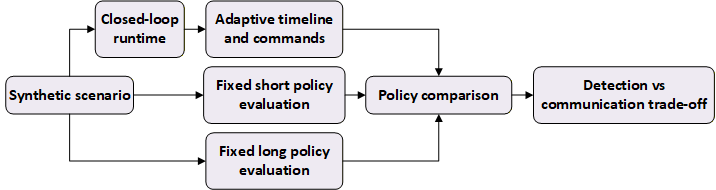
\includegraphics[width=\columnwidth]{fig/experimental_methodology2.png}
    \caption{Workflow of the comparative evaluation of the proposed framework.}
    \label{fig:experimental_methodology}
\end{figure}

\section{Results and Discussion}
\label{sec:Results_Discussion}
\subsection{Evidence of Closed-Loop Digital-Twin Execution}
In the reference execution reported in this work (the \textit{intermittent\_evening} scenario, seven days at native 5-minute resolution, fixed seed), the runtime traversed 2016 potential acquisition instants. Across this native-resolution timeline, the active observation mode was \textit{basal} for 1751 instants, \textit{moderate} for 168, and \textit{aggressive} for 97; under the resulting adaptive schedule with \textit{weighted} fusion, 299 instants were actually emitted and observed. In this same execution, 57 reconfiguration commands were issued, and 18 transport events fell back from NB-IoT to BLE. This evidence is architectural and operational, not merely classificatory: it demonstrates that the \textit{ForensicTwin}, \textit{DecisionEngine}, \textit{PolicyOrchestrator}, \textit{MockTransport}, and \textit{MockForensicDevice} were exercised as coupled components of a closed-loop architecture in which the observation process itself is a consequence of the twin's own decisions.

\subsection{Supervised Baseline: Accuracy, Discrimination, and Feature Importance}
On the same reference scenario, the logistic-regression baseline (1411 training and 605 held-out test instants, chronological split) achieved accuracy $0.9917$, precision $0.9298$, recall $0.9815$, F1-score $0.9550$, and AUROC $0.9948$. These values are high but, unlike results obtained before the realism corrections of Section~\ref{subsec:synthetic_realism}, are no longer at or extremely near the theoretical ceiling of $1.0000$ across every non-degenerate scenario, which is consistent with the classification task no longer being an artifact of the data-generation process. Fig.~\ref{fig:roc_curves} shows the corresponding ROC curve. A two-hidden-layer MLP trained on the same split achieved accuracy 0.9868, precision 0.9600, recall 0.8889, F1-score 0.9231, and AUROC 0.9981. The tested MLP did not improve the F1-score over logistic regression, suggesting that the additional nonlinear capacity considered here provided no clear advantage under this experimental configuration.

These are classifier-level diagnostics with every held-out instance available; unlike the policy-level metrics of Section~\ref{subsec:metrics}, they do not include observation-induced false negatives.

\begin{figure}[!ht]
    \centering
    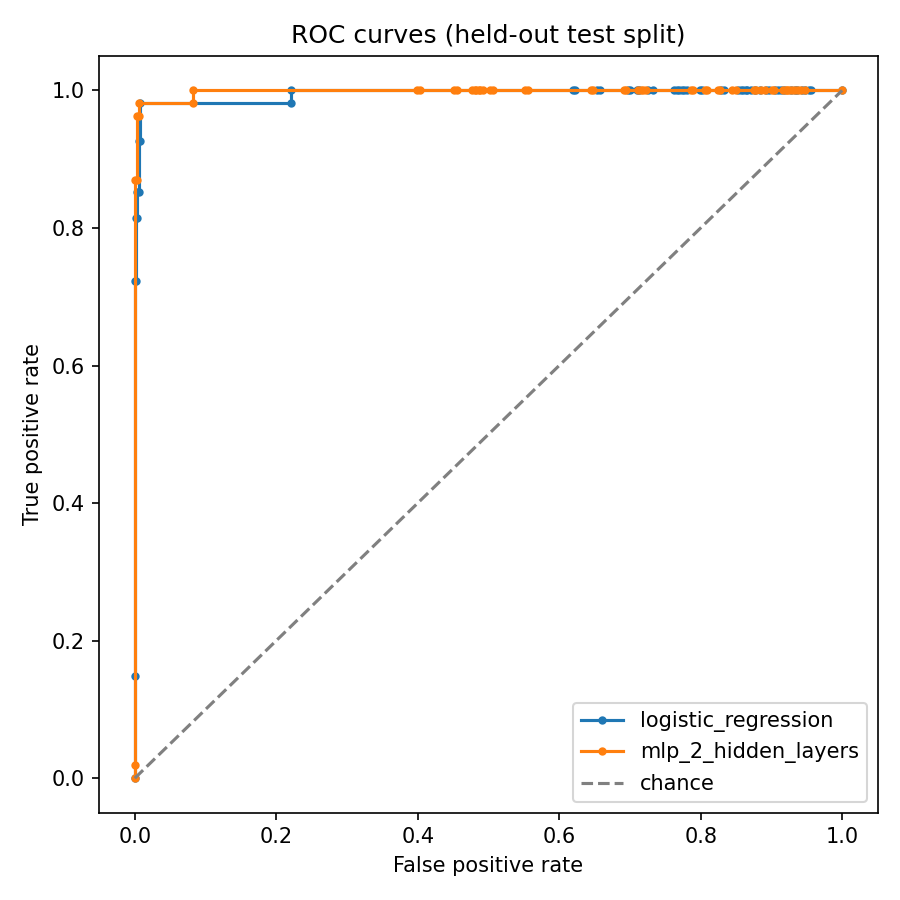
\includegraphics[width=\columnwidth]{fig/roc_curves.png}
    \caption{ROC curves for the logistic regression and MLP baselines on the held-out test split of the reference scenario.}
    \label{fig:roc_curves}
\end{figure}

Permutation importance (F1-scoring, 20 repetitions) on the held-out split ranks \texttt{relative\_divergence} as the dominant feature (mean importance $0.783$), followed by \texttt{alarm\_score} ($0.145$) and \texttt{slot\_recurrence} ($0.074$); the five remaining features each contribute less than $0.02$ of mean importance. Standardized logistic-regression coefficients follow the same ranking (\texttt{relative\_divergence}: $6.84$; \texttt{alarm\_score}: $2.03$; \texttt{slot\_recurrence}: $0.73$). This confirms that electrical divergence remains, as expected, the primary detection signal, but with a measurable and non-deterministic contribution rather than a one-to-one encoding of the label, and that the alarm and temporal-recurrence features contribute genuine secondary evidence rather than a redundant restatement of the same signal.

\subsection{Aggregate Performance Against the True Dense-Monitoring Ceiling}
\label{subsec:results_headline}
\begin{table}[ht]
\centering
\caption{Aggregate comparison across the seven-scenario campaign (mean values).}
\label{tab:agg_policy_results}
\scriptsize
\begin{tabular}{lcccc}
\hline
\textbf{Policy} & \textbf{Source/fusion} & \textbf{F1} & \textbf{Recall} & \textbf{Bytes} \\
\hline
\textit{fixed\_dense} & Supervised & 0.5545 & 0.5705 & 137{,}835 \\
\textit{fixed\_dense} & Rule-based & 0.5219 & 0.5467 & 137{,}835 \\
\textit{adaptive} & Decision / weighted & 0.5039 & 0.4727 & 40{,}646 \\
\textit{adaptive} & Supervised / weighted & 0.5024 & 0.4729 & 40{,}646 \\
\textit{adaptive} & Rule-based / weighted & 0.4805 & 0.4548 & 40{,}646 \\
\textit{fixed\_short} & Supervised & 0.2699 & 0.1814 & 47{,}621 \\
\textit{fixed\_short} & Rule-based & 0.2550 & 0.1735 & 47{,}621 \\
\textit{fixed\_long} & Supervised & 0.0822 & 0.0447 & 17{,}514 \\
\textit{fixed\_long} & Rule-based & 0.0784 & 0.0427 & 17{,}514 \\
\hline
\end{tabular}
\end{table}

Table~\ref{tab:agg_policy_results} reports the aggregate comparison across the full seven-scenario campaign, evaluated as described in Section~\ref{sec:experimental_campaign}. The \textit{fixed\_dense} policy, reporting at the native 5-minute resolution, is the correct empirical ceiling for ``what would detection performance be under the densest possible monitoring,'' and achieves a mean F1-score of $0.5545$ (supervised source) at a mean communication cost of $137{,}835$ bytes. The adaptive policy with \textit{weighted} fusion achieves a mean F1-score of $0.5039$ (decision probability) at $40{,}646$ bytes, retaining approximately $90.9\%$ of the dense-monitoring F1-score and $82.9\%$ of its recall while transmitting only approximately $29.5\%$ of the communication volume, a reduction of about $70.5\%$. This result holds consistently across probability sources: evaluating the same adaptive schedule under the supervised probability instead of the fused decision probability yields an essentially identical F1-score ($0.5024$) at the same communication cost, confirming that the benefit stems from the observation schedule itself rather than from a favorable choice of detection signal for one policy and not the others.

The mean values in Table~\ref{tab:scenario_breakdown} should not be interpreted as the detection quality attainable when theft is actually present, because three of the seven scenarios (\textit{normal}, \textit{disturbance\_without\_theft}, and \textit{degraded\_link\_no\_theft}) contain no theft instants by construction. Under the zero-value convention adopted in this evaluation for scenarios with no positive instances, these scenarios contribute zero precision, recall, and F1-score to the arithmetic mean. Table~\ref{tab:scenario_breakdown} therefore also reports the mean restricted to the four theft-bearing scenarios (\textit{persistent\_theft}, \textit{peak\_theft}, \textit{night\_theft}, and \textit{intermittent\_evening}). Under this restriction, the \textit{fixed\_dense} policy achieves a mean F1-score of 0.9703 and mean recall of 0.9984, while the adaptive policy achieves a mean F1-score of 0.8819 and mean recall of 0.8272.

Notably, the retention ratio between the adaptive policy and the dense-monitoring ceiling is essentially unchanged: approximately 90.9\% for F1-score and 82.9\% for recall in both the seven-scenario and four-theft-scenario computations. This occurs because the three theft-free scenarios contribute zero to both policies' detection metrics and therefore do not affect their ratio. We retain the seven-scenario mean as a campaign-wide aggregate for consistency across policies, but it should not be interpreted as a measure of performance on theft-free scenarios.

\begin{table*}[!ht]
\centering
\caption{Scenario-level detection performance and communication cost for the dense-monitoring ceiling and the adaptive policy.}
\label{tab:scenario_breakdown}
\begin{tabular}{lccccccc}
\hline
& & \multicolumn{3}{c}{\textit{fixed\_dense} (supervised)} & \multicolumn{3}{c}{\textit{adaptive} (weighted)} \\
\textbf{Scenario} & \textbf{Contains theft} & \textbf{F1} & \textbf{Recall} & \textbf{Bytes} & \textbf{F1} & \textbf{Recall} & \textbf{Bytes} \\
\hline
\textit{normal} & No & 0.0000 & 0.0000 & 135{,}452 & 0.0000 & 0.0000 & 17{,}736 \\
\textit{persistent\_theft} & Yes & 1.0000 & 1.0000 & 135{,}332 & 1.0000 & 1.0000 & 135{,}332 \\
\textit{peak\_theft} & Yes & 0.9264 & 0.9958 & 134{,}952 & 0.9159 & 0.8625 & 30{,}324 \\
\textit{night\_theft} & Yes & 0.9976 & 0.9976 & 135{,}152 & 0.9928 & 0.9881 & 41{,}884 \\
\textit{intermittent\_evening} & Yes & 0.9572 & 1.0000 & 135{,}212 & 0.6189 & 0.4581 & 25{,}204 \\
\textit{disturbance\_without\_theft} & No & 0.0000 & 0.0000 & 135{,}352 & 0.0000 & 0.0000 & 17{,}736 \\
\textit{degraded\_link\_no\_theft} & No & 0.0000 & 0.0000 & 153{,}396 & 0.0000 & 0.0000 & 16{,}304 \\
\hline
Mean, all 7 scenarios & --- & 0.5545 & 0.5705 & 137{,}835 & 0.5039 & 0.4727 & 40{,}646 \\
Mean, 4 theft-bearing scenarios & --- & 0.9703 & 0.9984 & 135{,}162 & 0.8819 & 0.8272 & 58{,}186 \\
\hline
\end{tabular}
\end{table*}

The scenario-level breakdown also identifies where the adaptive policy loses the most ground relative to the ceiling: in \textit{intermittent\_evening}, the campaign's most temporally erratic scenario (Section~\ref{subsec:synthetic_realism}), the adaptive policy's F1-score falls to $0.6189$ (recall $0.4581$), against $0.9572$ (recall $1.0000$) for \textit{fixed\_dense}, because the twin cannot always react in time to theft windows that activate unpredictably within a given evening. In \textit{peak\_theft} and \textit{night\_theft}, whose theft windows are temporally concentrated and therefore easier to anticipate once the twin has densified observation, the adaptive policy remains within about half a percentage point to about one percentage point of F1-score of the ceiling ($0.9928$ versus $0.9976$, and $0.9159$ versus $0.9264$, respectively) while using between $69\%$ and $78\%$ fewer bytes. This indicates that the aggregate retention figure reported above is not uniform across fraud behaviors, and that the adaptive policy's relative advantage is largest for temporally structured theft and smallest for highly erratic, short-notice theft.

The comparison against \textit{fixed\_short}, an intermediate 15-minute fixed cadence, is at least as informative: \textit{fixed\_short} is dominated by the adaptive policy in both dimensions simultaneously (F1-score $0.2699$ at a higher cost of $47{,}621$ bytes, versus F1-score $0.5039$ at $40{,}646$ bytes for the adaptive policy). This occurs because, once the native resolution was corrected (Section~\ref{subsec:native_resolution}), a fixed 15-minute cadence under-samples relative to the intermittent, short-lived fraud events represented in the campaign, while still incurring more communication cost than a policy that concentrates its (denser) sampling on the periods of elevated risk. The \textit{fixed\_long} policy, at the lowest cost ($17{,}514$ bytes), exhibits severe under-observation (F1-score $0.0822$, recall $0.0447$), confirming that permanently sparse monitoring is not a viable substitute for either dense or adaptive observation in this setting.

\subsection{Fusion-Strategy Ablation}
\label{subsec:results_fusion_ablation}
\begin{table}[ht]
\centering
\caption{Aggregate comparison of adaptive fusion strategies (mean, decision probability).}
\label{tab:agg_fusion_results}
\scriptsize
\begin{tabular}{lccc}
\hline
\textbf{Strategy} & \textbf{F1} & \textbf{Recall} & \textbf{Bytes} \\
\hline
\textit{weighted} & 0.5039 & 0.4727 & 40{,}646 \\
\textit{conservative\_max} & 0.4828 & 0.4694 & 41{,}105 \\
\textit{context\_aware} & 0.4714 & 0.4169 & 37{,}622 \\
\hline
\end{tabular}
\end{table}

Table~\ref{tab:agg_fusion_results} reports the aggregate comparison of the three fusion strategies. The \textit{weighted} strategy achieves the best mean F1-score. \textit{conservative\_max} is dominated by \textit{weighted} in both dimensions (lower F1-score at higher communication cost), confirming that inheriting the maximum of the two evidence sources over-amplifies isolated evidence into unnecessary densification without a corresponding detection benefit. \textit{context\_aware} trades approximately $6.4\%$ of the mean F1-score for an approximately $7.4\%$ reduction in communication cost relative to \textit{weighted}, which is a genuine, interpretable trade-off rather than a strict dominance in either direction; this indicates that the added semantic sophistication of context-dependent weighting did not, in this campaign, translate into a Pareto improvement over the simpler weighted combination, and that further refinement of the context-switching rules (Section~\ref{subsec:fusao}) would need to specifically target detection performance, not only cost, to outperform the weighted baseline outright.

\subsection{Critical-Slot Metric: Binary and Relaxed}
The binary critical-slot-hit metric is $0.5714$ (mean fraction of scenarios hit) for the adaptive policy and as low as $0.2857$ for \textit{fixed\_dense} under the rule-based source, despite the latter having a higher raw F1-score in that configuration; the relaxed score of Eq.~\eqref{eq:relaxed_critical_slot} resolves this apparent inconsistency, reporting $0.9496$ for the adaptive policy and $0.5394$ for \textit{fixed\_dense} (rule-based), which indicates that even the ``misses'' recorded by the binary metric were, on average, temporally close to the true busiest theft hour for the adaptive policy but more temporally dispersed for \textit{fixed\_dense} under the rule-based source. This confirms the value of reporting both metrics together, as recommended by the temporal-tolerance evaluation literature \cite{b36,b37}: the binary metric flags whether the policy achieved exact temporal precision, while the relaxed metric quantifies how operationally close a non-exact result still was.

\subsection{Communication-Cost Trade-off Resolution}
\label{subsec:results_pareto}
The grid search of Section~\ref{subsec:tradeoff_resolution} evaluated 60 configurations of $(\alpha, \tau_{\text{moderate}}, \tau_{\text{high}})$ on three representative scenarios, of which 30 aggregate configurations are non-dominated in the $\bigl(F_1, C\bigr)$ plane. Fig.~\ref{fig:pareto_frontier} shows the resulting frontier. The configuration used elsewhere in this paper ($\alpha = 0.6$, $\tau_{\text{moderate}} = 0.30$, $\tau_{\text{high}} = 0.60$) achieves F1-score $0.869$ at a mean cost of $30{,}635$ bytes on this three-scenario subset; it lies close to, but not exactly on, the empirical frontier, whose nearest point at comparable cost ($\tau_{\text{high}} = 0.50$, all else equal) achieves F1-score $0.878$ at $30{,}751$ bytes, a difference of about one percentage point of F1-score at essentially the same communication cost. This is reported as an honest empirical characterization of the operating point actually used, rather than as a retroactive re-tuning of production defaults based on a three-scenario grid: the frontier is offered as a decision-support artifact for selecting an operating point according to deployment-specific preferences, consistent with the framing of Section~\ref{sec:system_model}.

\begin{figure}[!ht]
    \centering
    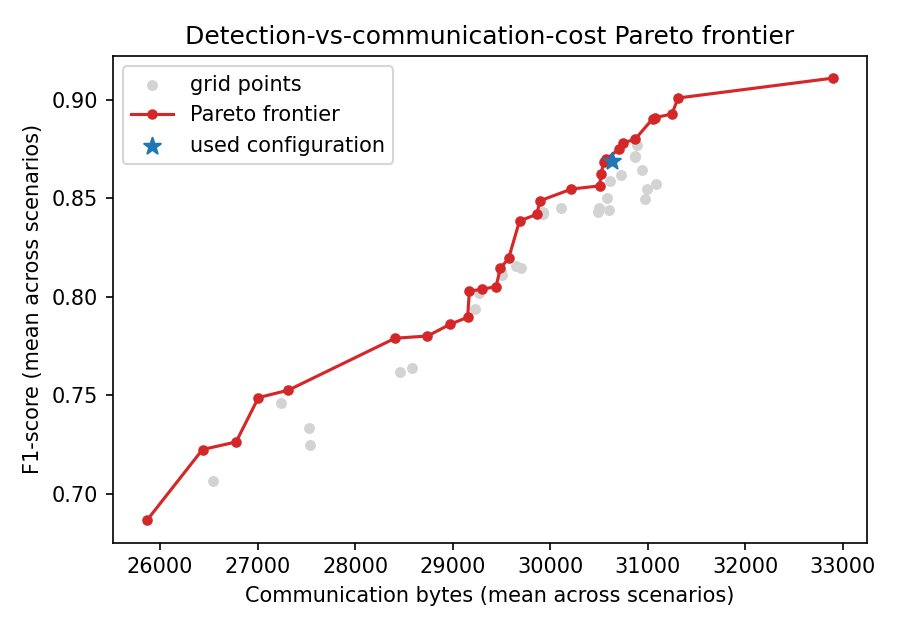
\includegraphics[width=\columnwidth]{fig/policy_pareto_frontier.png}
    \caption{Empirical Pareto frontier between detection (F1-score) and communication cost, obtained by grid search over the fusion weight and hysteresis thresholds. The star marks the configuration used elsewhere in this paper.}
    \label{fig:pareto_frontier}
\end{figure}

\subsection{Computational Complexity and Scalability}
\label{subsec:results_scalability}
Fig.~\ref{fig:scalability} reports the wall-clock time per twin and peak memory usage as the number of sequentially processed twins grows from 1 to 100, each replaying the same 2016-event trace. Across the tested fleet sizes, the measured per-twin processing time remains approximately constant, ranging from $0.999$~s for a single twin to $1.051$~s for 100 twins, corresponding to a drift ratio of $1.05\times$ across two orders of magnitude in fleet size. Peak memory remains between $9.85$ and $10.34$~MB throughout. These measurements are consistent with the $O(N\cdot T)$ sequential-complexity analysis of Section~\ref{subsec:complexity} and indicate that no additional fleet-size-dependent processing overhead emerged within the evaluated single-process benchmark.

\begin{figure}[!ht]
    \centering
    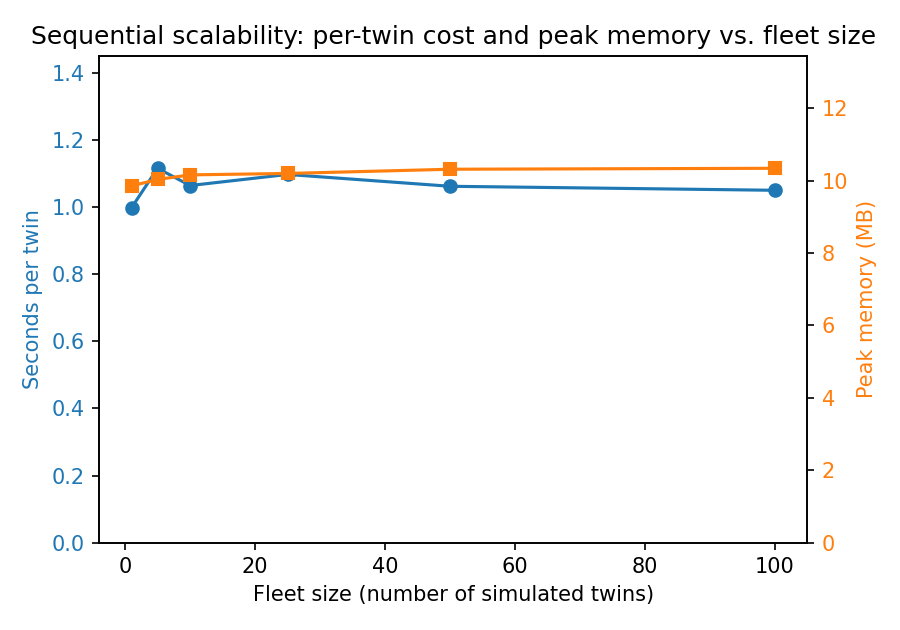
\includegraphics[width=\columnwidth]{fig/scalability_benchmark.png}
    \caption{Sequential wall-clock cost per twin and peak memory usage as a function of fleet size.}
    \label{fig:scalability}
\end{figure}

Taken together, the experiments validate the closed-loop implementation, quantify the detection--communication and scalability trade-offs, and preserve traceability from twin state and commands to the reported artifacts.

\subsection{Threats to Validity and Limitations}
\label{subsec:limitations}
Several limitations constrain the scope of the conclusions that can be drawn from this study, and are stated explicitly rather than left implicit. First, and most importantly, validation relies entirely on synthetic scenarios. However, a distribution utility partner already collects field forensic-telemetry data of the kind targeted by this framework; that data is presently subject to an ongoing forensic and legal evaluation process to support corrective action against customers with indications of fraud, and cannot yet be disclosed for research publication. Consequently, this study validates the framework's internal coherence and behavior under controlled, heterogeneous synthetic conditions. It identifies field-data validation as the primary direction for future work, not an omission. Second, the physical bidirectional synchronization criterion of Section~\ref{subsec:twin_criteria} is satisfied only in a local, reproducible simulation; end-to-end integration with a deployed NB-IoT/BLE radio link remains future work, and the communication-cost model, while grounded in reported measurement studies (Section~\ref{subsec:network_cost}), is not itself a field measurement. Third, the Pareto-frontier analysis of Section~\ref{subsec:tradeoff_resolution} restricts the search to a three-parameter hysteresis-policy family evaluated on three scenarios for computational tractability; it resolves the trade-off empirically within that family but does not constitute a proof of global optimality over the full action-sequence space of Section~\ref{sec:system_model}, and a sequential decision-making formulation (e.g., a partially observable Markov decision process solved by reinforcement learning, as has been explored for related adaptive-sampling and theft-detection problems \cite{b38}) is a natural extension for removing this restriction. Fourth, the \textit{context\_aware} fusion strategy did not outperform the simpler \textit{weighted} strategy in this campaign (Section~\ref{subsec:results_fusion_ablation}); this is reported as a negative result rather than omitted, and indicates that the value of contextual fusion depends on further refinement of its switching rules. Fifth, the computational-scalability benchmark of Section~\ref{subsec:results_scalability} evaluates a single-process, sequential execution and should therefore be interpreted as a characterization of computational scaling within that implementation model. A production deployment could exploit parallel execution across independent twins, potentially improving throughput; however, shared-resource contention, communication, storage, and orchestration overheads may also affect scalability and were not evaluated in this study. Sixth, the synthetic campaign uses deterministic fixed-seed realizations rather than repeated simulations across multiple random seeds. The reported performance values therefore characterize the specific controlled traces used in this study and are not accompanied by between-realization confidence intervals; multi-seed evaluation is left for future work.


\section{Conclusion}
\label{sec:Conclusion}
This work demonstrated that an application-oriented digital twin can use contextual theft-risk estimates to adapt the observation window of NB-IoT forensic telemetry, formalizing detection capability and communication cost as explicit functions of the twin's observational state and selected action, and resolving their trade-off empirically through a Pareto-frontier analysis rather than through unjustified fixed weights. Across a seven-scenario experimental campaign built with heterogeneous fraud severities, independent measurement and communication noise, and a native acquisition resolution fine enough to make every observation mode operationally distinguishable, the adaptive policy retained approximately 91\% of the F1-score and 83\% of the recall of the true dense-monitoring ceiling while transmitting approximately 30\% of the communication volume, and dominated an intermediate fixed-cadence baseline in both detection and cost simultaneously. A communication-cost model grounded in reported NB-IoT quality-of-service measurements, a feature-importance and alternative-model analysis, a relaxed temporal-tolerance metric, and a computational-scalability benchmark consistent with linear sequential scaling complement these findings.

Beyond these numerical results, the study shows a conceptual shift from static classification to adaptive observation control, with the digital twin operating as an explicit-state, closed-loop decision layer whose label criteria are stated and checked individually rather than asserted. The framework's physical bidirectional synchronization is, at present, closed only in a local, reproducible simulation, and its detection-versus-cost trade-off is resolved within a restricted, interpretable policy family; field-data validation, end-to-end NB-IoT/BLE integration, and a sequential decision-making formulation of the observation policy are identified as the primary directions for future work. Contextual risk-driven adaptation is a technically coherent and quantitatively characterized strategy for forensic telemetry in communication-constrained smart-metering environments.

\section*{Data Availability}
This paper describes the underlying prototype as reproducible, based on its deterministic synthetic-data generation, its explicit twin-state and command-plan traceability artifacts (Section~\ref{sec:Materials_Methods}), and the fact that every table and figure in Section~\ref{sec:Results_Discussion} is produced by a documented, script-driven pipeline rather than by manual computation. At the time of this submission, however, we had not yet established a public code repository or dataset deposit. The full source code, including the digital-twin components (\textit{ForensicTwin}, \textit{DecisionEngine}, \textit{PolicyOrchestrator}), the synthetic-data generator, the mock device/transport/billing-meter simulators, and the analysis scripts used for the Pareto-frontier and scalability results, together with the synthetic datasets and generated artifacts underlying every reported number, is available from the corresponding author upon request.

\section*{Acknowledgment}
This work was supported in part by the Coordenação de Aperfeiçoamento de Pessoal de Nível Superior (CAPES), Brazil, Finance Code 001, and by the Programa de Excelência Acadêmica (PROEX). The authors also acknowledge the Núcleo de Estudos e Pesquisas do Norte e Nordeste (NEPEN), Instituto Constanta de Inovação (ICI), and EDP South America for providing the infrastructure and material resources essential to this research, conducted under ANEEL R\&D project PD-00391-0054/25. The authors used ChatGPT (OpenAI) to help generate the conceptual illustration shown in Fig.~\ref{fig:use_case_topology}. The authors reviewed and edited the resulting figure and take full responsibility for its content.

\begin{thebibliography}{00}

\bibitem{b1}
P. Jeyaraj, E. Nadar, A. Kathiresan, and S. Asokan,
``Smart grid security enhancement by detection and classification of non-technical losses employing deep learning algorithm,''
\textit{Int. Trans. Electr. Energy Syst.},
vol. 30, no. 9, Art. no. e12521, 2020,
doi: 10.1002/2050-7038.12521.

\bibitem{b2}
M. Hasan, R. Toma, A.-A. Nahid, M. Islam, and J.-M. Kim,
``Electricity theft detection in smart grid systems: A CNN-LSTM based approach,''
\textit{Energies},
vol. 12, no. 17, Art. no. 3310, 2019,
doi: 10.3390/en12173310.

\bibitem{b3}
H. Gul, N. Javaid, I. Ullah, A. Qamar, M. Afzal, and G. Joshi,
``Detection of non-technical losses using SOSTLink and bidirectional gated recurrent unit to secure smart meters,''
\textit{Appl. Sci.},
vol. 10, no. 9, Art. no. 3151, 2020,
doi: 10.3390/app10093151.

\bibitem{b4}
A. Kawoosa, D. Prashar, M. Faheem, N. Jha, and A. Khan,
``Using machine learning ensemble method for detection of energy theft in smart meters,''
\textit{IET Gener. Transm. Distrib.},
vol. 17, no. 21, pp. 4794--4809, 2023,
doi: 10.1049/gtd2.12997.

\bibitem{b5}
M. Hashim, L. Khan, N. Javaid, Z. Ullah, and A. Javed,
``Stacked machine learning models for non-technical loss detection in smart grid: A comparative analysis,''
\textit{Energy Rep.},
vol. 12, pp. 1235--1253, 2024,
doi: 10.1016/j.egyr.2024.06.015.

\bibitem{b6}
A. Massarani, M. Badr, M. Baza, H. Alshahrani, and A. Alshehri,
``Efficient and accurate zero-day electricity theft detection from smart meter sensor data using prototype and ensemble learning,''
\textit{Sensors},
vol. 25, no. 13, Art. no. 4111, 2025,
doi: 10.3390/s25134111.

\bibitem{b7}
M. Gunduz and R. Das,
``Smart grid security: An effective hybrid CNN-based approach for detecting energy theft using consumption patterns,''
\textit{Sensors},
vol. 24, no. 4, Art. no. 1148, 2024,
doi: 10.3390/s24041148.

\bibitem{b8}
A. Ali, L. Khan, N. Javaid, S. Bouk, A. Aldegheishem, and N. Alrajeh,
``Mitigating anomalous electricity consumption in smart cities using an AI-based stacked-generalization technique,''
\textit{IET Renew. Power Gener.},
vol. 19, no. 1, Art. no. e12785, 2025,
doi: 10.1049/rpg2.12785.

\bibitem{b9}
T. Mu, Y. Yu, G. Feng, H. Luo, and H. Yang,
``Detecting anomalous electricity consumption with transformer and synthesized anomalies,''
\textit{PeerJ Comput. Sci.},
vol. 9, Art. no. e1721, 2023,
doi: 10.7717/peerj-cs.1721.

\bibitem{b10}
M. Žarković and G. Dobrić,
``Artificial intelligence for energy theft detection in distribution networks,''
\textit{Energies},
vol. 17, no. 7, Art. no. 1580, 2024,
doi: 10.3390/en17071580.

\bibitem{b11}
J. Vasantrao and C. Patel,
``AT\&C and non-technical loss reduction in smart grid using smart metering with AI techniques,''
\textit{The Scientific Temper},
vol. 16, no. 8, pp. 4635--4645, 2025,
doi: 10.58414/SCIENTIFICTEMPER.2025.16.8.06.

\bibitem{b12}
K. Blazakis, N. Schetakis, M. Badr, D. Aghamalyan, K. Stavrakakis, and G. Stavrakakis,
``Power theft detection in smart grids using quantum machine learning,''
\textit{IEEE Access},
vol. 13, pp. 61511--61525, 2025,
doi: 10.1109/ACCESS.2025.3558143.

\bibitem{b13}
A. Maamar and K. Benahmed,
``A hybrid model for anomaly detection in AMI system combining K-means clustering and deep neural network,''
\textit{Comput. Mater. Continua},
vol. 60, no. 1, pp. 15--39, 2019,
doi: 10.32604/cmc.2019.06497.

\bibitem{b14}
A. Kawoosa et al.,
``Improving electricity theft detection using electricity information collection system and customers' consumption patterns,''
\textit{Energy Explor. Exploit.},
vol. 42, no. 5, pp. 1684--1714, 2024,
doi: 10.1177/01445987241255394.

\bibitem{b15}
M. Callcut, J.-P. Cerceau Agliozzo, L. Varga, and L. McMillan,
``Digital twins in civil infrastructure systems,''
\textit{Sustainability},
vol. 13, no. 20, Art. no. 11549, 2021,
doi: 10.3390/su132011549.

\bibitem{b16}
M. Dihan et al.,
``Digital twin: Data exploration, architecture, implementation and future,''
\textit{Heliyon},
vol. 10, no. 5, Art. no. e26503, 2024,
doi: 10.1016/j.heliyon.2024.e26503.

\bibitem{b17}
A. Somma, D. Amalfitano, A. De Benedictis, and P. Pelliccione,
``TwinArch: A digital twin reference architecture,''
\textit{J. Syst. Softw.},
vol. 231, Art. no. 112613, 2026,
doi: 10.1016/j.jss.2025.112613.

\bibitem{b18}
M. Elsisi, K. Mahmoud, M. Lehtonen, and M. Darwish,
``Reliable Industry 4.0 based on machine learning and IoT for analyzing, monitoring, and securing smart meters,''
\textit{Sensors},
vol. 21, no. 2, Art. no. 487, 2021,
doi: 10.3390/s21020487.

\bibitem{b19}
M. Habib et al.,
``Smart meter development using digital twin technology for green energy distribution optimization,''
\textit{European Journal of Theoretical and Applied Sciences},
vol. 1, no. 3, pp. 181--190, 2023,
doi: 10.59324/ejtas.2023.1(3).20.

\bibitem{b20}
M. Irfan, A. Niaz, M. Habib, M. Shoukat, S. Atta, and A. Ali,
``Digital twin concept, method and technical framework for smart meters,''
\textit{European Journal of Theoretical and Applied Sciences},
vol. 1, no. 3, pp. 105--117, 2023,
doi: 10.59324/ejtas.2023.1(3).10.

\bibitem{b21}
F. Han, F. Du, S. Jiao, and K. Zou,
``Predictive analysis of a building's power consumption based on digital twin platforms,''
\textit{Energies},
vol. 17, no. 15, Art. no. 3692, 2024,
doi: 10.3390/en17153692.

\bibitem{b22}
M. Bin Zaheen, R. Arshad, A. Ul Ain, A. Sarwar, and M. Khan,
``Digital twin-based smart metering framework with real-time monitoring via Microsoft Azure IoT,''
in \textit{Proc. 20th Int. Conf. Emerging Technol. (ICET)},
2025, pp. 1--7,
doi: 10.1109/ICET66147.2025.11321353.

\bibitem{b23}
M. Mahmoodian, F. Shahrivar, S. Setunge, and S. Mazaheri,
``Development of digital twin for intelligent maintenance of civil infrastructure,''
\textit{Sustainability},
vol. 14, no. 14, Art. no. 8664, 2022,
doi: 10.3390/su14148664.

\bibitem{b24}
P. Almasan et al.,
``Digital twin network: Opportunities and challenges,''
\textit{arXiv preprint arXiv:2201.01144}, 2022,
doi: 10.48550/arXiv.2201.01144.

\bibitem{b25}
H. Liu et al.,
``Research on intelligent control technology for a rail-based high-throughput crop phenotypic platform based on digital twins,''
\textit{Agriculture},
vol. 15, no. 11, Art. no. 1217, 2025,
doi: 10.3390/agriculture15111217.

\bibitem{b26}
S. Qaddoori and Q. Ali,
``An embedded and intelligent anomaly power consumption detection system based on smart metering,''
\textit{IET Wirel. Sens. Syst.},
vol. 13, no. 2, pp. 75--90, 2023,
doi: 10.1049/wss2.12054.

\bibitem{b27}
M. Raeiszadeh, A. Ebrahimzadeh, R. Glitho, J. Eker, and R. Mini,
``Real-time adaptive anomaly detection in industrial IoT environments,''
\textit{IEEE Trans. Netw. Service Manag.},
vol. 21, no. 6, pp. 6839--6856, 2024,
doi: 10.1109/TNSM.2024.3447532.

\bibitem{b28}
A. El Sayed, M. Ruiz, H. Harb, and L. Velasco,
``Deep learning-based adaptive compression and anomaly detection for smart B5G use cases operation,''
\textit{Sensors},
vol. 23, no. 2, Art. no. 1043, 2023,
doi: 10.3390/s23021043.

\bibitem{b29}
K. Al-Sammak et al.,
``Optimizing IoT energy efficiency: Real-time adaptive algorithms for smart meters with LoRaWAN and NB-IoT,''
\textit{Energies},
vol. 18, no. 4, Art. no. 987, 2025,
doi: 10.3390/en18040987.

\bibitem{b30}
X. Fan, C. Zhou, Y. Sun, J. Du, and Y. Zhao,
``Research on remote meter reading scheme and IoT smart energy meter based on NB-IoT technology,''
\textit{J. Phys.: Conf. Ser.},
vol. 1187, no. 2, Art. no. 022064, 2019,
doi: 10.1088/1742-6596/1187/2/022064.

\bibitem{b31}
M. Maduranga and A. Wijerathna,
``NB-IoT based status measurement system for 33 kV power distribution networks in smart grids,''
\textit{International Journal of Engineering and Manufacturing},
vol. 12, no. 4, pp. 37--45, 2022,
doi: 10.5815/ijem.2022.04.04.

\bibitem{b32}
A. Sultania, F. Mahfoudhi, and J. Famaey,
``Real-time demand response using NB-IoT,''
\textit{IEEE Internet Things J.},
vol. 7, no. 12, pp. 11863--11872, 2020,
doi: 10.1109/JIOT.2020.3004390.

\bibitem{b33}
M. Stusek et al.,
``Exploiting NB-IoT network performance and capacity for smart-metering use-cases,''
in \textit{Proc. 15th Int. Congr. Ultra Modern Telecommunications and Control Systems and Workshops (ICUMT)},
2023, pp. 193--199,
doi: 10.1109/ICUMT61075.2023.10333294.

\bibitem{b34}
A. P. Matz, J.-A. Fernández-Prieto, J. Cañada-Bago, and U. Birkel,
``A systematic analysis of Narrowband IoT quality of service,''
\textit{Sensors},
vol. 20, no. 6, Art. no. 1636, 2020,
doi: 10.3390/s20061636.

\bibitem{b35}
A. Sultania, C. Blondia, and J. Famaey,
``Optimizing the energy-latency trade-off in NB-IoT with PSM and eDRX,''
\textit{IEEE Internet Things J.},
vol. 8, no. 15, pp. 12436--12454, 2021,
doi: 10.1109/JIOT.2021.3063435.

\bibitem{b36}
R. Salles et al.,
``SoftED: Metrics for soft evaluation of time series event detection,''
\textit{Comput. Ind. Eng.},
vol. 198, Art. no. 110728, 2024,
doi: 10.1016/j.cie.2024.110728.

\bibitem{b37}
E. Scharwächter and E. Müller,
``Statistical evaluation of anomaly detectors for sequences,''
\textit{arXiv preprint arXiv:2008.05788}, 2020,
doi: 10.48550/arXiv.2008.05788.

\bibitem{b38}
A. El-Toukhy, M. Badr, M. Mahmoud, G. Srivastava, M. Fouda, and M. Alsabaan,
``Electricity theft detection using deep reinforcement learning in smart power grids,''
\textit{IEEE Access},
vol. 11, pp. 59558--59574, 2023,
doi: 10.1109/ACCESS.2023.3284681.


\bibitem{b39}
L. Liu, Y. Ding, X. Li, H. Wu, and L. Xing,
``A container-driven service architecture to minimize the upgrading requirements of user-side smart meters in distribution grids,''
\textit{IEEE Trans. Ind. Informat.},
vol. 18, no. 1, pp. 719--728, Jan. 2022,
doi: 10.1109/TII.2021.3088135.

\bibitem{b40}
D. Bayer and M. Pruckner,
``A digital twin of a local energy system based on real smart meter data,''
\textit{Energy Informatics},
vol. 6, Art. no. 8, 2023,
doi: 10.1186/s42162-023-00263-6.

\end{thebibliography}

\begin{biography}[{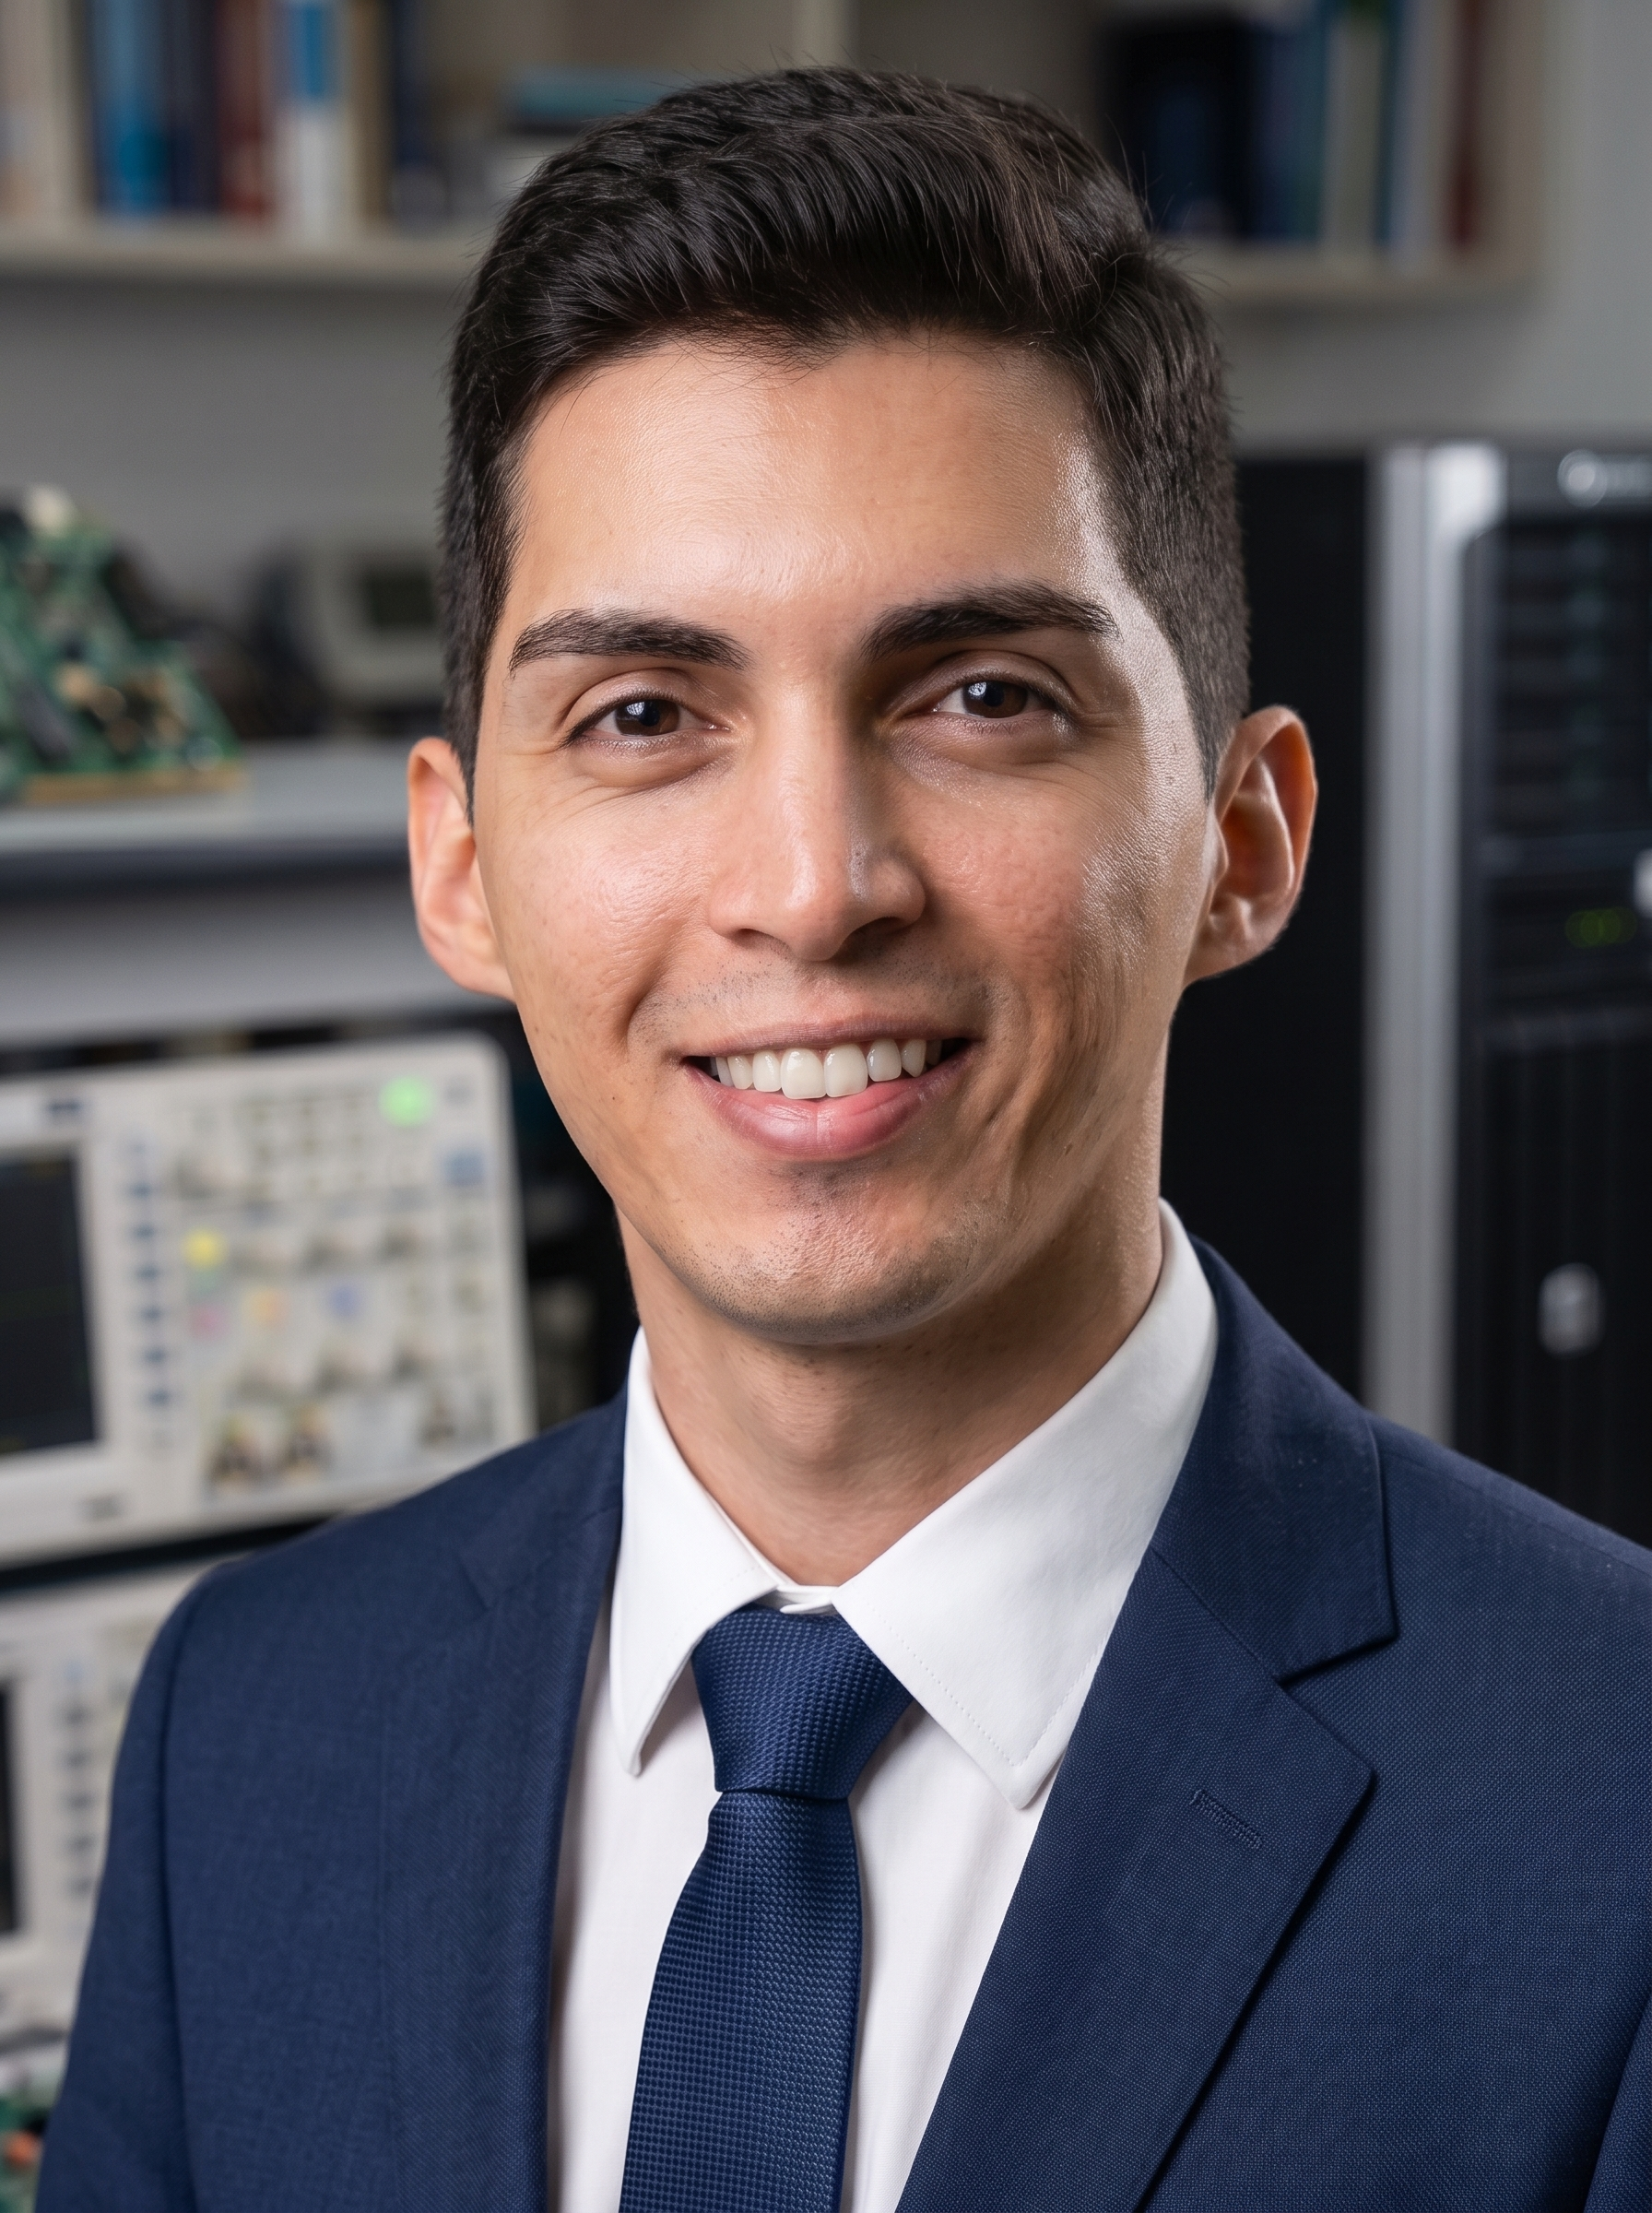
\includegraphics[width=1in,height=1.25in,clip,keepaspectratio]{fig/Coutinho.png}}]{Danilo Coutinho Filho}
received the M.S. degree in teleinformatics engineering from the Federal University of Ceará (UFC), Brazil, in 2023. He is currently pursuing the Ph.D. degree in teleinformatics engineering at UFC. He is a Researcher at the Engineering Laboratory of Computer Systems (LESC Lab) and the Center for Studies and Research of the North and Northeast (NEPEN), and has served as a Guest Reviewer for the IEEE Open Journal of the Communications Society.
\end{biography}

\begin{biography}[{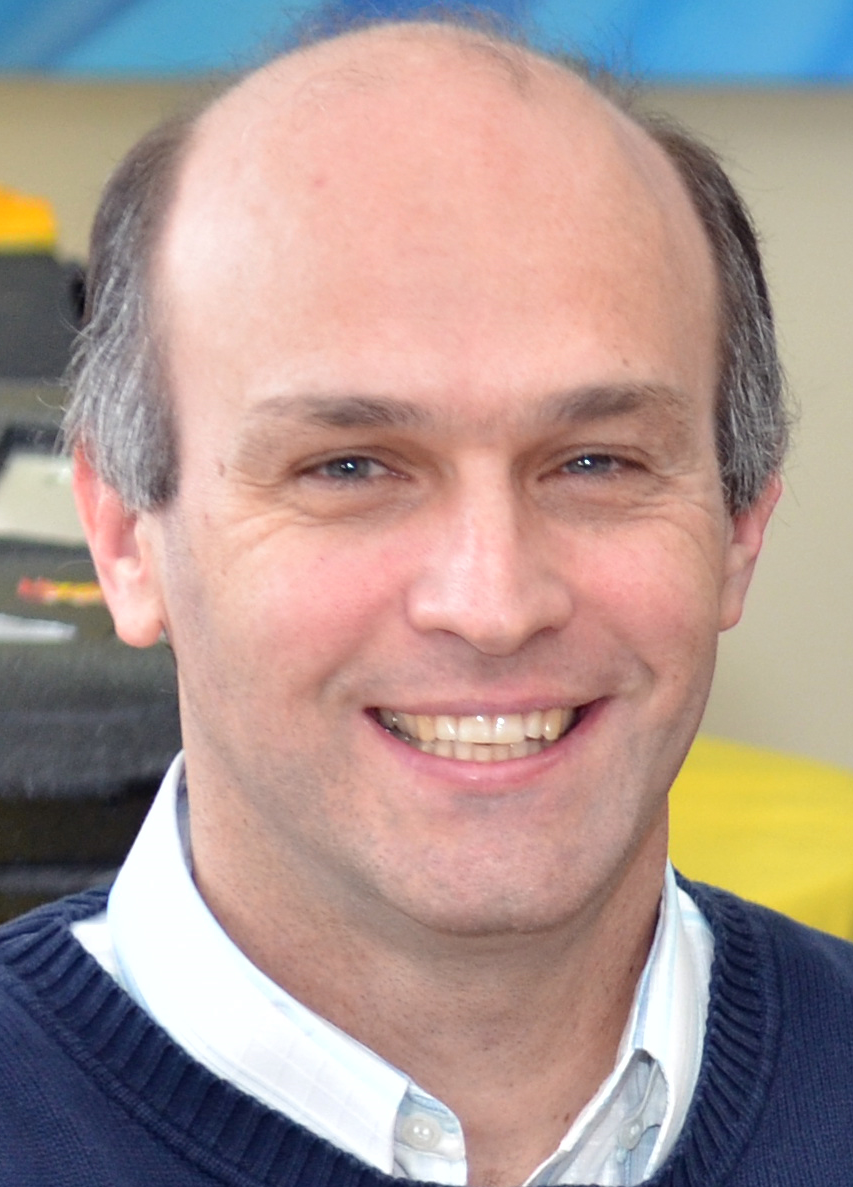
\includegraphics[width=1in,height=1.25in,clip,keepaspectratio]{fig/Cesar_Marcon.png}}]{César Marcon}
(Senior Member, IEEE) received the Ph.D. degree in computer science from the Federal University of Rio Grande do Sul (UFRGS), Brazil, in 2005. He has been a Professor at the Polytechnic School of the Pontifical Catholic University of Rio Grande do Sul (PUCRS), Brazil, since 1995. He is a distinguished Brazilian researcher with a CNPq PQ grant.
\end{biography}

\begin{biography}[{
\includegraphics[width=1in,height=1.25in,clip,keepaspectratio]{fig/Jarbas_Silveira.jpg}}]{Jarbas Silveira}
(Senior Member, IEEE) received the Ph.D. degree in teleinformatics engineering from the Federal University of Ceará (UFC), Brazil, in 2015. He has been an Adjunct Professor in the Teleinformatics Department at UFC since 2009, where he is also affiliated with the Engineering Laboratory of Computer Systems (LESC Lab). He is a distinguished Brazilian researcher with a CNPq PQ grant.
\end{biography}

\begin{biography}[{
\includegraphics[width=1in,height=1.25in,clip,keepaspectratio]{fig/Diógenes.png}}]{Rogério Diógenes Filho}
received the B.Sc. and M.Sc. degrees in Telecommunications Engineering from the Federal Institute of Ceará (IFCE), Brazil, in 2013 and 2016, respectively, and a specialization degree in Technological Innovation in 2015. He is a Professor at IFCE and currently serves as Director of Innovation at NEPEN and the Constanta Institute of Innovation. He has more than 15 years of experience in research, development, and innovation, with emphasis on Smart Grids, Internet of Things (IoT), embedded systems, LoRaWAN, NB-IoT, and private LTE/5G networks. He is an inventor of seven patents and has led large-scale innovation projects involving smart metering, interoperable communication devices, IoT networks, and private cellular infrastructure, including the deployment of a private LTE/5G network for CELESC to support mission-critical utility applications.
\end{biography}

\begin{biography}[{
\includegraphics[width=1in,height=1.25in,clip,keepaspectratio]{fig/Matos.png}}]{Michel Matos}
received the B.Sc. degree in Electrical Engineering from the Universidade Cruzeiro do Sul, São Paulo, Brazil, in 2018, and the M.B.A. degree in Project Management from Fundação Getulio Vargas (FGV), São Paulo, Brazil, in 2020. He is currently a Project Management Specialist in Research and Development at EDP, Brazil, where he leads engineering studies and research and development projects focused on technological transformation and innovation in electric power distribution systems.
\end{biography}

\EOD

\end{document}
